%%%%%%%%%%%%%%%%%%%%%%%%%%%%%%%%%%%%%%%%%%%%%%%%%%%
%% LaTeX book template                           %%
%% Author:  Amber Jain (http://amberj.devio.us/) %%
%% License: ISC license                          %%
%%%%%%%%%%%%%%%%%%%%%%%%%%%%%%%%%%%%%%%%%%%%%%%%%%%

\documentclass[a4paper,11pt,oneside]{book}
\usepackage{modulestyle}

%%%%%%%%%%%%%%%%%%%%%%%%%%%%%%%%%%%%%%%%%%%%%%%%%%%%%%%%%
% Source: http://en.wikibooks.org/wiki/LaTeX/Hyperlinks %
%%%%%%%%%%%%%%%%%%%%%%%%%%%%%%%%%%%%%%%%%%%%%%%%%%%%%%%%%

%%%%%%%%%%%%%%%%%%%%%%%%%%%%%%%%%%%%%%%%%%%%%%%%%%%%%%%%%%%%%%%%%%%%%%%%%%%%%%%%
% 'dedication' environment: To add a dedication paragraph at the start of book %
% Source: http://www.tug.org/pipermail/texhax/2010-June/015184.html            %
%%%%%%%%%%%%%%%%%%%%%%%%%%%%%%%%%%%%%%%%%%%%%%%%%%%%%%%%%%%%%%%%%%%%%%%%%%%%%%%%
\newenvironment{dedication}
{
   \cleardoublepage
   \thispagestyle{empty}
   \vspace*{\stretch{1}}
   \hfill\begin{minipage}[t]{0.66\textwidth}
   \raggedright
}
{
   \end{minipage}
   \vspace*{\stretch{3}}
   \clearpage
}

%%%%%%%%%%%%%%%%%%%%%%%%%%%%%%%%%%%%%%%%%%%%%%%%
% Chapter quote at the start of chapter        %
% Source: http://tex.stackexchange.com/a/53380 %
%%%%%%%%%%%%%%%%%%%%%%%%%%%%%%%%%%%%%%%%%%%%%%%%
\makeatletter
\renewcommand{\@chapapp}{}% Not necessary...
\newenvironment{chapquote}[2][2em]
  {\setlength{\@tempdima}{#1}%
   \def\chapquote@author{#2}%
   \parshape 1 \@tempdima \dimexpr\textwidth-2\@tempdima\relax%
   \itshape}
  {\par\normalfont\hfill--\ \chapquote@author\hspace*{\@tempdima}\par\bigskip}
\makeatother

%%%%%%%%%%%%%%%%%%%%%%%%%%%%%%%%%%%%%%%%%%%%%%%%%%%
% First page of book which contains 'stuff' like: %
%  - Book title, subtitle                         %
%  - Book author name                             %
%%%%%%%%%%%%%%%%%%%%%%%%%%%%%%%%%%%%%%%%%%%%%%%%%%%

\newcommand{\BookTitle}{Object-Oriented Programming}
\newcommand{\BookTitleFootnote}{A course in the Bachelor of Science in Computer
Science}

\newcommand{\BookSubtitle}{A Study Guide for Students of Sorsogon State University - Bulan Campus}
\newcommand{\BookSubtitleFootnote}{This book is a study guide for students of
Sorsogon State University - Bulan Campus taking up the course Object-Oriented
Programming.}

\newcommand{\BookAuthorFirstName}{Jarrian Vince}
\newcommand{\BookAuthorLastName}{Gojar}
\newcommand{\BookAuthorName}{Jarrian Vince G. Gojar}
\newcommand{\BookAuthorURL}{https://github.com/godkingjay}

% Book's title and subtitle
\title{\Huge \textbf{\BookTitle}  \footnote{\BookTitleFootnote} \\
\huge \BookSubtitle \footnote{\BookSubtitleFootnote}}

% Author
\author{\textsc{\BookAuthorName}\thanks{\url{\BookAuthorURL}}}

\begin{document}

\frontmatter
\maketitle

%%%%%%%%%%%%%%%%%%%%%%%%%%%%%%%%%%%%%%%%%%%%%%%%%%%%%%%%%%%%%%%
% Add a dedication paragraph to dedicate your book to someone %
%%%%%%%%%%%%%%%%%%%%%%%%%%%%%%%%%%%%%%%%%%%%%%%%%%%%%%%%%%%%%%%
\begin{dedication}
Sorsogon State University - Bulan Campus
\end{dedication}

%%%%%%%%%%%%%%%%%%%%%%%%%%%%%%%%%%%%%%%%%%%%%%%%%%%%%%%%%%%%%%%%%%%%%%%%
% Auto-generated table of contents, list of figures and list of tables %
%%%%%%%%%%%%%%%%%%%%%%%%%%%%%%%%%%%%%%%%%%%%%%%%%%%%%%%%%%%%%%%%%%%%%%%%
\tableofcontents
\listoffigures
\listoftables
\lstlistoflistings

\mainmatter

%%%%%%%%%%%
% Preface %
%%%%%%%%%%%
\chapter*{Preface}
\begin{chapquote}{Dennis Ritchie}
``The only way to learn a new programming language is by writing programs in it.''
\end{chapquote}

\noindent \BookAuthorName \\
\noindent \url{\BookAuthorURL}

%%%%%%%%%%%%%%%%%%%%%%%
%%%     Chapter     %%%
%%%%%%%%%%%%%%%%%%%%%%%
\chapter{Introduction to Java Programming Language and Object-Oriented Programming}

% \begin{chapquote}{James Gosling}
% ``Java is a general-purpose, concurrent, class-based, object-oriented programming
% language that was designed and developed by Sun Microsystems in the early 1990s.''
% \end{chapquote}

\section{Introduction}

Java is a general-purpose, concurrent, class-based, object-oriented programming
language that was designed and developed by Sun Microsystems in the early 1990s.
It is currently owned by Oracle Corporation. Java is one of the most popular
programming languages in use, particularly for client-server web applications.

\subsection{History of Java}

Before Java, the primary programming language was C++. C++ is a powerful
programming language, but it is complex and difficult to learn. It is also
platform-dependent, which means that C++ programs must be recompiled for each
operating system. Java was designed to be easy to use and is therefore easier to
write, compile, debug, and learn than C++.

Java was developed by James Gosling, Mike Sheridan, and Patrick Naughton at Sun
Microsystems in the early 1990s. It was first released in 1995 as a core
component of Sun Microsystems' Java platform. The language derives much of its
syntax from C and C++, but it has fewer low-level facilities than either of
them.

The original and reference implementation Java compilers, virtual machines, and
class libraries were developed by Sun from 1991 and first released in 1995. As
of May 2007, in compliance with the specifications of the Java Community
Process, Sun made available most of their Java technologies as free software
under the GNU General Public License. Sun's vice-president Rich Green said that
Sun's ideal role with regard to Java was as an evangelist.

Sun Microsystems released the first public implementation as Java 1.0 in 1995.
It promised Write Once, Run Anywhere (WORA), providing no-cost run-times on
popular platforms. Fairly secure and featuring configurable security, it allowed
network- and file-access restrictions. Major web browsers soon incorporated the
ability to run Java applets within web pages, and Java quickly became popular.

In 2006, for marketing purposes, Sun renamed new J2 versions as Java EE, Java ME,
and Java SE, respectively.

In 2006, Sun released much of its Java virtual machine (JVM) as free and open-source
software (FOSS), under the terms of the GNU General Public License (GPL). Sun's
software strategy had been to use the language to sell hardware, so FOSS would
have put Sun at a disadvantage.

After Oracle Corporation acquired Sun in 2009, Oracle has described itself as the
``steward of Java technology with a relentless commitment to fostering a community
of participation and transparency''.

In 2011, Oracle Corporation sued Google for having distributed a new implementation
of Java embedded in the Android operating system. Google had not acquired any
licenses from Sun or Oracle. The American court system ruled in favor of Google
stating that the implementation of Java in Android was considered fair use.

In September 2017, Mark Reinhold, chief Architect of the Java Platform, proposed
to change the release train to ``one feature release every six months''. Therefore,
Oracle announced that it would be moving away from a release model that
produces a major release every two years, and instead moving to a model that
produces a feature release every six months. The first version was released in
March 2018.

In 2019, the Oracle Corporation announced that it would be moving Java EE to the
Eclipse Foundation, to make the process of developing Java EE faster, more agile,
and more open.

In recent years, Java has been one of the most popular programming languages in
use, particularly for client-server web applications, with a reported 9 million
developers.

As of today, Java is one of the most popular programming languages in use,
particularly for client-server web applications.

\subsection{Java Virtual Machine(JVM)}

The Java Virtual Machine (JVM) is an abstract computing machine that enables a
computer to run a Java program. There are three notions of the JVM: specification,
implementation, and instance. The specification is a document that formally
describes what is required of a JVM implementation. Having a single specification
ensures all implementations are interoperable. A JVM implementation is a computer
program that meets the requirements of the JVM specification. An instance of a
JVM is an implementation running in a process that executes a computer program
compiled into Java bytecode.

\subsection{Java Development Kit(JDK)}

The Java Development Kit (JDK) is a software development kit used to develop Java
applications and applets. It is one of the most widely used Java software
development kits. It consists of the Java Runtime Environment (JRE), an interpreter/loader
(Java), a compiler (javac), an archiver (jar), a documentation generator (Javadoc),
and other tools needed in Java development.

To install the JDK, you need to download the JDK from the Oracle website. You
can download the JDK from the following URL: \url{https://www.oracle.com/ph/java/technologies/downloads/}

\subsection{Java IDE (Integrated Development Environment)}

An Integrated Development Environment (IDE) is a software application that
provides comprehensive facilities to computer programmers for software development.
An IDE normally consists of a source code editor, build automation tools, and a
debugger. Most modern IDEs have intelligent code completion.

There are many IDEs available for Java development. Some of the most popular
IDEs are:

\begin{multicols*}{2}
  \begin{itemize}
    \item Eclipse
    \item NetBeans
    \item IntelliJ IDEA
    \item JDeveloper
    \item BlueJ
    \item DrJava
    \item JCreator
    \item JGrasp
    \item MyEclipse
    \item Oracle JDeveloper
    \item Visual Studio Code
    \item Xcode
    \item Android Studio
    \item Code::Blocks
    \item CodeLite
  \end{itemize}
\end{multicols*}

One of the most popular IDEs for Java development is Eclipse. Eclipse is an
integrated development environment (IDE) used in computer programming. It contains
a base workspace and an extensible plug-in system for customizing the environment.
Eclipse is written mostly in Java and its primary use is for developing Java
applications, but it may also be used to develop applications in other programming
languages through the use of plugins, including Ada, ABAP, C, C++, and more.

To install Eclipse, you need to download the Eclipse IDE from the Eclipse website.
You can download Eclipse from the following URL:
\url{https://www.eclipse.org/downloads/}

\subsection{Summary}

Java is a general-purpose, concurrent, class-based, object-oriented programming
language that was designed and developed by Sun Microsystems in the early 1990s.
It is currently owned by Oracle Corporation. Java is one of the most popular
programming languages in use, particularly for client-server web applications.

\section{Basic Syntax}

Java is a case-sensitive language. This means that the language keywords,
variables, function names, and any other identifiers must always be typed
with a consistent capitalization of letters. The following are the keywords
in Java.These are reserved words that have special meaning to the compiler
and cannot be used for other purposes:

\begin{multicols}{4}
  \begin{itemize}
    \item abstract
    \item assert
    \item boolean
    \item break
    \item byte
    \item case
    \item catch
    \item char
    \item class
    \item const
    \item continue
    \item default
    \item do
    \item double
    \item else
    \item enum
    \item extends
    \item final
    \item finally
    \item float
    \item for
    \item goto
    \item if
    \item implements
    \item import
    \item instanceof
    \item int
    \item interface
    \item long
    \item native
    \item new
    \item package
    \item private
    \item protected
    \item public
    \item return
    \item short
    \item static
    \item strictfp
    \item super
    \item switch
    \item synchronized
    \item this
    \item throw
    \item throws
    \item transient
    \item try
    \item void
    \item volatile
    \item while
  \end{itemize}
\end{multicols}

\subsection{Java Program Structure}

A Java program is a collection of classes. A class is a blueprint from which
objects are created. A class can contain fields (variables) and methods (functions).
A Java program must have a class definition. A class definition includes the
following components:

\begin{multicols*}{3}
  \begin{itemize}
    \item Modifiers
    \item Class name
    \item Superclass (if any)
    \item Interfaces (if any)
    \item Body
    \item Fields
    \item Methods
    \item Constructors
    \item Blocks
    \item Nested classes and interfaces
    \item Annotations
    \item Comments
    \item Package statement
    \item Import statement
    \item Main method
    \item Statements and expressions
    \item Variables
    \item Literals
    \item Arrays
    \item Enumerations
  \end{itemize}
\end{multicols*}

\begin{lstlisting}[language=Java, caption={Basic Syntax of a Java Program}]
  // BasicSyntax.java
  package com.oop.BasicSyntax;
  
  public class BasicSyntax {
    public static void main(String[] args) {
      System.out.println("This is the basic syntax of Java programming language.");
    }
  }
\end{lstlisting}

The code above shows the basic syntax of a Java program. The program prints the
message ``This is the basic syntax of Java programming language.''

\subsubsection{package}

\begin{lstlisting}[language=Java, caption={Package Declaration}]
  package com.oop.BasicSyntax;
\end{lstlisting}

The line `package com.oop.BasicSyntax;` in Java is used to declare the package to
which the current Java file belongs. In this case, the Java file is part of the
`com.oop.BasicSyntax` package. Packages are used to organize classes and interfaces
into namespaces, making it easier to manage and maintain large Java projects.

The package declaration must be the first line in a Java file, and it is optional.
If a package declaration is not included in a Java file, the file is considered to
be part of the default package.

The package name must be a valid Java identifier, and it should follow the Java
naming conventions. The package name can be a simple name or a compound name
separated by periods. For example, `com.oop.BasicSyntax` is a simple package name,
and `com.oop.BasicSyntax.util` is a compound package name.

The package has the following syntax:

\begin{itemize}
  \item \textnormal{[package] [package\_name];}
\end{itemize}

The package declaration includes the following components:

\begin{itemize}
  \item \textnormal{package: The keyword that indicates the start of the package declaration.}
  \item \textnormal{[package\_name]: The name of the package to which the Java file belongs.}
\end{itemize}

\subsubsection{class}

\begin{lstlisting}[language=Java, caption={Class Declaration}]
  public class BasicSyntax {
    // Class body
  }
\end{lstlisting}

The line ``public class BasicSyntax \{\}'' in Java is used to declare a class named
``BasicSyntax''. A class is a blueprint for creating objects in Java. It defines the
structure and behavior of objects by specifying fields (variables) and methods

The class has the following syntax:

\begin{itemize}
  \item \textnormal{[access\_modifier] class [class\_name] \{ [class\_body] \}}
\end{itemize}

The code block inside the class is called the class body. The class body contains
the fields, methods, constructors, and other components of the class.

The class declaration has the following components:

\begin{itemize}
  \item \textnormal{[access\_modifier]: The access modifier that specifies the visibility
  of the class.}
  \item \textnormal{class: The keyword that indicates the start of the class declaration.}
  \item \textnormal{[class\_name]: The name of the class. The class name should be a valid
  Java identifier.}
  \item \textnormal{\{ [class\_body] \}: The code block inside the class. The class body
  contains the fields, methods, constructors, and other components of the class.}
\end{itemize}

The classes in Java can have the following access modifiers:

\begin{itemize}
  \item \textnormal{public: The class is accessible by any other class.}
  \item \textnormal{protected: The class is accessible by classes in the same package and
  subclasses in other packages.}
  \item \textnormal{default: The class is accessible only by classes in the same package.}
  \item \textnormal{private: The class is accessible only within the same class.}
  \item \textnormal{final: The class cannot be subclassed.}
  \item \textnormal{abstract: The class cannot be instantiated.}
  \item \textnormal{strictfp: The class follows the strict floating-point rules defined by
  the IEEE 754 standard.}
\end{itemize}

For coding conventions, the class name should be a valid Java identifier, and it
should follow the Java naming conventions. The class name should be in CamelCase
format, starting with an uppercase letter.

The class body is enclosed in curly braces \{\}. The class body contains the
fields, methods, constructors, and other components of the class.

\subsubsection{main method}

\begin{lstlisting}[language=Java, caption={Main Method or Driver Method}]
  public static void main(String[] args) {
    // Method body
  }
\end{lstlisting}

The line ``public static void main(String[] args) \{\}'' in Java is used to declare
the main method of the class. The main method is the entry point of a Java program.
When a Java program is executed, the main method is called by the Java Virtual
Machine (JVM) to start the program.

The main method has the following syntax:

\begin{itemize}
  \item \textnormal{public static void main(String[] args) \{ [method\_body] \}}
\end{itemize}

The main method is a special method in Java that has the following components:

\begin{itemize}
  \item \textnormal{public: The access modifier that indicates the main method is accessible
  by any other class.}
  \item \textnormal{static: The keyword that indicates the main method belongs to the class
  and not to the instance of the class.}
  \item \textnormal{void: The return type of the main method. The main method does not return
  any value.}
  \item \textnormal{main: The name of the main method. The main method is the entry point of
  a Java program.}
  \item \textnormal{String[] args: The parameter of the main method. The args parameter is an
  array of strings that stores the command-line arguments passed to the Java program.}
  \item \textnormal{[method\_body]: The code block inside the main method. The method body
  contains the statements and expressions that define the behavior of the main method.}
\end{itemize}

The main method is the entry point of a Java program. When a Java program is executed,
the Java Virtual Machine (JVM) calls the main method to start the program.

\begin{lstlisting}[language=Java, caption={Print Message to Console}]
  System.out.println("This is the basic syntax of Java programming language.");
\end{lstlisting}

The line ``System.out.println("This is the basic syntax of Java programming language.");''
in Java is used to print a message to the console. The ``System.out.println()'' method
is used to print a message to the standard output stream (console).

The ``System.out.println()'' method has the following syntax:

\begin{itemize}
  \item \textnormal{System.out.println([message]);}
\end{itemize}

It has the following components:

\begin{itemize}
  \item \textnormal{System: The class name. The System class is a predefined class in Java
  that provides access to the system resources.}
  \item \textnormal{out: The static field of the System class. The out field is an instance
  of the PrintStream class that provides methods to write data to the standard output
  stream (console).}
  \item \textnormal{println(): The method of the PrintStream class. The println() method is
  used to print a message to the standard output stream (console).}
  \item \textnormal{[message]: The message to be printed. The message can be a string, a
  number, or any other value that can be converted to a string.}
\end{itemize}

\subsection{Summary}

The basic syntax of a Java program includes the package declaration, class
declaration, and main method. The package declaration is used to declare the
package to which the Java file belongs. The class declaration
is used to declare a class in Java. The main method is the entry point of a Java
program and is called by the Java Virtual Machine (JVM) to start the program.

\section{Lexical Structure}

The lexical structure of a programming language defines the set of valid tokens
that can be used to write programs in the language. The lexical structure of Java
includes the following elements:

\begin{itemize}
  \item \textnormal{Unicode: Java programs are written using the Unicode character
  set, which supports a wide range of characters from different languages.}
  \item \textnormal{Lexical Translations: Java programs are translated into Unicode
  characters using the Unicode escape sequences.}
  \item \textnormal{Unicode Escapes: Unicode escape sequences are used to represent
  Unicode characters in Java programs.}
  \item \textnormal{Line Terminators: Line terminators are used to mark the end of a
  line in a Java program.}
  \item \textnormal{Input Elements and Tokens: Input elements are the smallest
  individual units of a Java program, and tokens are the meaningful sequences of
  input elements.}
  \item \textnormal{White Space: White space characters are used to separate tokens
  and improve the readability of a Java program.}
  \item \textnormal{Comments: Comments are used to document Java programs and improve
  their readability.}
  \item \textnormal{Identifiers: Identifiers are used to name classes, methods,
  variables, and other elements in a Java program.}
  \item \textnormal{Keywords: Keywords are reserved words in Java that have special
  meanings and cannot be used as identifiers.}
  \item \textnormal{Literals: Literals are fixed values that are used in Java programs,
  such as numbers, characters, and strings.}
  \item \textnormal{Separators: Separators are used to separate tokens in a Java
  program, such as parentheses, braces, and commas.}
  \item \textnormal{Operators: Operators are used to perform operations on operands in
  a Java program, such as addition, subtraction, and comparison.}
\end{itemize}

\subsection{Unicode}

Unicode is a character encoding standard that supports a wide range of
characters from different languages and scripts. Java programs are written
using the Unicode character set, which allows developers to use characters
from various languages in their code.

Unicode escape sequences are used to represent Unicode characters in Java
programs. For example, the Unicode escape sequence \textnormal{\textbackslash{u0041}} represents
the character 'A' in the Latin alphabet.

\begin{lstlisting}[language=Java, caption={Unicode Character}]
  char unicodeCharacter = '\u0041';
	System.out.println("Unicode Character: " + unicodeCharacter);
\end{lstlisting}

The code above declares a variable named \textnormal{unicodeCharacter} of type
\textnormal{char} and assigns the Unicode character \textnormal{\textbackslash{u0041}}
to it. The code then prints the Unicode character 'A' to the console.

Read more about Unicode at \url{https://unicode.org/}

% These are some of the Unicode escape sequences from 32 to 127

% \begin{multicols*}{4}
%   \begin{itemize}
%     \item \textnormal{\textbackslash{u0020}}: Space
%     \item \textnormal{\textbackslash{u0021}}: !
%     \item \textnormal{\textbackslash{u0022}}: "
%     \item \textnormal{\textbackslash{u0023}}: \#
%     \item \textnormal{\textbackslash{u0024}}: \$
%     \item \textnormal{\textbackslash{u0025}}: \%
%     \item \textnormal{\textbackslash{u0026}}: \&
%     \item \textnormal{\textbackslash{u0027}}: '
%     \item \textnormal{\textbackslash{u0028}}: (
%     \item \textnormal{\textbackslash{u0029}}: )
%     \item \textnormal{\textbackslash{u002A}}: *
%     \item \textnormal{\textbackslash{u002B}}: +
%     \item \textnormal{\textbackslash{u002C}}: ,
%     \item \textnormal{\textbackslash{u002D}}: -
%     \item \textnormal{\textbackslash{u002E}}: .
%     \item \textnormal{\textbackslash{u002F}}: /
%     \item \textnormal{\textbackslash{u0030}}: 0
%     \item \textnormal{\textbackslash{u0031}}: 1
%     \item \textnormal{\textbackslash{u0032}}: 2
%     \item \textnormal{\textbackslash{u0033}}: 3
%     \item \textnormal{\textbackslash{u0034}}: 4
%     \item \textnormal{\textbackslash{u0035}}: 5
%     \item \textnormal{\textbackslash{u0036}}: 6
%     \item \textnormal{\textbackslash{u0037}}: 7
%     \item \textnormal{\textbackslash{u0038}}: 8
%     \item \textnormal{\textbackslash{u0039}}: 9
%     \item \textnormal{\textbackslash{u003A}}: :
%     \item \textnormal{\textbackslash{u003B}}: ;
%     \item \textnormal{\textbackslash{u003C}}: <
%     \item \textnormal{\textbackslash{u003D}}: =
%     \item \textnormal{\textbackslash{u003E}}: >
%     \item \textnormal{\textbackslash{u003F}}: ?
%     \item \textnormal{\textbackslash{u0040}}: @
%     \item \textnormal{\textbackslash{u0041}}: A
%     \item \textnormal{\textbackslash{u0042}}: B
%     \item \textnormal{\textbackslash{u0043}}: C
%     \item \textnormal{\textbackslash{u0044}}: D
%     \item \textnormal{\textbackslash{u0045}}: E
%     \item \textnormal{\textbackslash{u0046}}: F
%     \item \textnormal{\textbackslash{u0047}}: G
%     \item \textnormal{\textbackslash{u0048}}: H
%     \item \textnormal{\textbackslash{u0049}}: I
%     \item \textnormal{\textbackslash{u004A}}: J
%     \item \textnormal{\textbackslash{u004B}}: K
%     \item \textnormal{\textbackslash{u004C}}: L
%     \item \textnormal{\textbackslash{u004D}}: M
%     \item \textnormal{\textbackslash{u004E}}: N
%     \item \textnormal{\textbackslash{u004F}}: O
%     \item \textnormal{\textbackslash{u0050}}: P
%     \item \textnormal{\textbackslash{u0051}}: Q
%     \item \textnormal{\textbackslash{u0052}}: R
%     \item \textnormal{\textbackslash{u0053}}: S
%     \item \textnormal{\textbackslash{u0054}}: T
%     \item \textnormal{\textbackslash{u0055}}: U
%     \item \textnormal{\textbackslash{u0056}}: V
%     \item \textnormal{\textbackslash{u0057}}: W
%     \item \textnormal{\textbackslash{u0058}}: X
%     \item \textnormal{\textbackslash{u0059}}: Y
%     \item \textnormal{\textbackslash{u005A}}: Z
%     \item \textnormal{\textbackslash{u005B}}: [
%     \item \textnormal{\textbackslash{u005C}}: \textbackslash
%     \item \textnormal{\textbackslash{u005D}}: ]
%     \item \textnormal{\textbackslash{u005E}}: \^{}
%     \item \textnormal{\textbackslash{u005F}}: \_
%     \item \textnormal{\textbackslash{u0060}}: `
%     \item \textnormal{\textbackslash{u0061}}: a
%     \item \textnormal{\textbackslash{u0062}}: b
%     \item \textnormal{\textbackslash{u0063}}: c
%     \item \textnormal{\textbackslash{u0064}}: d
%     \item \textnormal{\textbackslash{u0065}}: e
%     \item \textnormal{\textbackslash{u0066}}: f
%     \item \textnormal{\textbackslash{u0067}}: g
%     \item \textnormal{\textbackslash{u0068}}: h
%     \item \textnormal{\textbackslash{u0069}}: i
%     \item \textnormal{\textbackslash{u006A}}: j
%     \item \textnormal{\textbackslash{u006B}}: k
%     \item \textnormal{\textbackslash{u006C}}: l
%     \item \textnormal{\textbackslash{u006D}}: m
%     \item \textnormal{\textbackslash{u006E}}: n
%     \item \textnormal{\textbackslash{u006F}}: o
%     \item \textnormal{\textbackslash{u0070}}: p
%     \item \textnormal{\textbackslash{u0071}}: q
%     \item \textnormal{\textbackslash{u0072}}: r
%     \item \textnormal{\textbackslash{u0073}}: s
%     \item \textnormal{\textbackslash{u0074}}: t
%     \item \textnormal{\textbackslash{u0075}}: u
%     \item \textnormal{\textbackslash{u0076}}: v
%     \item \textnormal{\textbackslash{u0077}}: w
%     \item \textnormal{\textbackslash{u0078}}: x
%     \item \textnormal{\textbackslash{u0079}}: y
%     \item \textnormal{\textbackslash{u007A}}: z
%     \item \textnormal{\textbackslash{u007B}}: \{
%     \item \textnormal{\textbackslash{u007C}}: |
%     \item \textnormal{\textbackslash{u007D}}: \}
%     \item \textnormal{\textbackslash{u007E}}: \textasciitilde
%     \item \textnormal{\textbackslash{u007F}}: \textbackslash{u007F}
%   \end{itemize}
% \end{multicols*}

\subsection{Line Terminators}

Line terminators are used to mark the end of a line in a Java program. The
line terminator can be a carriage return (CR), a line feed (LF), or a
carriage return followed by a line feed (CRLF).

The line terminator is used to separate lines of code in a Java program and
improve the readability of the code.

\begin{itemize}
  \item \textnormal{CR (Carriage Return): Moves the cursor to the beginning of the line.}
  \item \textnormal{LF (Line Feed): Moves the cursor to the next line.}
  \item \textnormal{CRLF (Carriage Return Line Feed): Moves the cursor to the beginning
  of the next line.}
\end{itemize}

\begin{lstlisting}[language=Java, caption={Line Terminators}]
  // Carriage Return (CR)
  System.out.print("Hello, World!\r");

  // Line Feed (LF)
  System.out.print("Hello, World!\n");

  // Carriage Return Line Feed (CRLF)
  System.out.print("Hello, World!\r\n");
\end{lstlisting}

The code above demonstrates the use of line terminators in Java. The code prints
the message ``Hello, World!'' to the console using different line terminators.

\subsection{White Space}

White space characters are used to separate tokens in a Java program and improve
the readability of the code. White space characters include spaces, tabs, and
line terminators.

White space is ignored by the Java compiler, so developers can use it liberally
to format their code and make it more readable.

\begin{lstlisting}[language=Java, caption={Using White Space to Improve Readability}]
  // Using White Space to Improve Readability
  int number = 10;
  int result = number * 2;
  System.out.println("Result: " + result);

  if (result > 10) {
    System.out.println("Result is greater than 10");
  } else {
    System.out.println("Result is less than or equal to 10");
  }
\end{lstlisting}

The code above demonstrates the use of white space characters in Java. The code
uses spaces and line breaks to format the code and make it more readable.

\begin{lstlisting}[language=Java, caption={Code Without White Space}]
int number=10;int result=number*2;System.out.println("Result: "+result);if(result>10){System.out.println("Result is greater than 10");}else{System.out.println("Result is less than or equal to 10");}
\end{lstlisting}

The code above is the same as the previous code but without white space characters.
The code is difficult to read and understand because it lacks proper formatting.

\subsection{Comments}

Comments are used to document Java programs and improve their readability. Comments
are ignored by the Java compiler and are not executed as part of the program.

There are three types of comments in Java:

\begin{itemize}
  \item \textnormal{Single-Line Comments: Single-line comments start with // and continue
  until the end of the line.}
  \item \textnormal{Multi-Line Comments: Multi-line comments start with /* and end with *\/.
  They can span multiple lines.}
  \item \textnormal{Javadoc Comments: Javadoc comments start with /** and end with *\/. They
  are used to generate documentation from the source code.}
\end{itemize}

Comments are an essential part of writing maintainable code, as they help other
developers understand the purpose and functionality of the code.

\subsection{Identifiers}

Identifiers are used to name classes, methods, variables, and other elements in
a Java program. Identifiers must follow certain rules and conventions:

\begin{itemize}
  \item \textnormal{An identifier can only contain letters, digits, underscores (\_), and
  dollar signs (\$).}
  \item \textnormal{An identifier must start with a letter, underscore, or dollar sign.}
  \item \textnormal{Identifiers are case-sensitive, so uppercase and lowercase letters are
  considered different.}
  \item \textnormal{Identifiers should be descriptive and follow the naming conventions of
  the Java programming language.}
\end{itemize}

Good identifiers help make the code more readable and maintainable by providing
meaningful names for the elements in the program.

\begin{lstlisting}[language=Java, caption={Valid and Invalid Identifiers}]
  // Valid Identifiers
  int number;
  String firstName;
  double averageScore;
  boolean isComplete;
  void printMessage();

  // Invalid Identifiers
  int 1number; // Cannot start with a digit
  String first-name; // Cannot contain hyphens
  double average score; // Cannot contain spaces
  boolean isComplete?; // Cannot contain special characters
  void print Message(); // Cannot contain spaces
\end{lstlisting}

The code above demonstrates valid and invalid identifiers in Java. Valid identifiers
follow the rules and conventions of the Java programming language, while invalid
identifiers violate these rules.

\subsection{Keywords}

Keywords are reserved words in Java that have special meanings and cannot be used
as identifiers. Keywords are an essential part of the Java programming language
and are used to define the syntax and structure of Java programs.

The following are the keywords in Java:

\begin{multicols}{4}
  \begin{itemize}
    \item abstract
    \item assert
    \item boolean
    \item break
    \item byte
    \item case
    \item catch
    \item char
    \item class
    \item const
    \item continue
    \item default
    \item do
    \item double
    \item else
    \item enum
    \item extends
    \item final
    \item finally
    \item float
    \item for
    \item goto
    \item if
    \item implements
    \item import
    \item instanceof
    \item int
    \item interface
    \item long
    \item native
    \item new
    \item package
    \item private
    \item protected
    \item public
    \item return
    \item short
    \item static
    \item strictfp
    \item super
    \item switch
    \item synchronized
    \item this
    \item throw
    \item throws
    \item transient
    \item try
    \item void
    \item volatile
    \item while
  \end{itemize}
\end{multicols}

Keywords are an essential part of the Java programming language and are used to
define the syntax and structure of Java programs. They have special meanings and
cannot be used as identifiers.

\subsection{Literals}

Literals are fixed values that are used in Java programs. There are several types
of literals in Java:

\begin{itemize}
  \item \textnormal{Integer Literals: Integer literals are whole numbers without a decimal point.}
  \item \textnormal{Floating-Point Literals: Floating-point literals are numbers with a
  decimal point or an exponent.}
  \item \textnormal{Character Literals: Character literals are single characters enclosed
  in single quotes.}
  \item \textnormal{String Literals: String literals are sequences of characters enclosed
  in double quotes.}
  \item \textnormal{Boolean Literals: Boolean literals are either true or false.}
  \item \textnormal{Null Literal: The null literal represents the absence of a value.}
\end{itemize}

Literals are used to represent fixed values in Java programs and are an essential
part of writing code.

\begin{lstlisting}[language=Java, caption={Literals in Java}]
  // Integer Literal
  int integerLiteral = 10;
  System.out.println("Integer Literal: " + integerLiteral);

  // Floating-Point Literal
  double floatingPointLiteral = 3.14;
  System.out.println("Floating-Point Literal: " + floatingPointLiteral);

  // Character Literal
  char characterLiteral = 'A';
  System.out.println("Character Literal: " + characterLiteral);

  // String Literal
  String stringLiteral = "Hello, World!";
  System.out.println("String Literal: " + stringLiteral);

  // Boolean Literal
  boolean booleanLiteral = true;
  System.out.println("Boolean Literal: " + booleanLiteral);

  // Null Literal
  Object nullLiteral = null;
  System.out.println("Null Literal: " + nullLiteral);
\end{lstlisting}

The code above demonstrates the use of literals in Java. The code declares variables
of different types and assigns them literal values. The code then prints the
variables to the console.

\subsection{Separators}

Separators are used to separate tokens in a Java program. The following are the
separators in Java:

\begin{itemize}
  \item \textnormal{Parentheses: ( )}
  \item \textnormal{Braces: \{ \}}
  \item \textnormal{Brackets: [ ]}
  \item \textnormal{Semicolon: ;}
  \item \textnormal{Comma: ,}
  \item \textnormal{Period: .}
  \item \textnormal{Ellipsis: ...}
\end{itemize}

Separators are an essential part of the Java syntax and are used to define the
structure of Java programs.

\begin{lstlisting}[language=Java, caption={Separators in Java}]
  public class Separators {
    public static void main(String[] args) {
      // Using Parentheses to Group Expressions
      int result1 = (10 + 5) * 2;
      System.out.println("Result 1: " + result1);

      // Using Braces to Define
      if (result1 > 10) {
        System.out.println("Result 1 is greater than 10");
      } else {
        System.out.println("Result 1 is less than or equal to 10");
      }

      // Using Brackets to Access Array Elements
      int[] numbers = { 1, 2, 3, 4, 5 };
      System.out.println("First Element: " + numbers[0]);

      // Using Semicolon to Terminate Statements
      int x = 10;
      int y = 20;
      int z = x + y;
      System.out.println("Sum: " + z);

      // Using Comma to Separate Variables
      int a = 1, b = 2, c = 3;
      System.out.println("Values: " + a + ", " + b + ", " + c);

      // Using Period to Access Members
      String text = "Hello, World!";
      int length = text.length();
      System.out.println("Length: " + length);

      // Using Ellipsis to Indicate Variable Arguments
      int sum = add(1, 2, 3, 4, 5);
      System.out.println("Sum: " + sum);
    }

    /**
    * Method to Calculate the Sum of Variable Arguments
    * 
    * @param numbers the variable arguments to be added
    * @return the sum of the variable arguments
    */
    public static int add(int... numbers) {
      int sum = 0;
      for (int number : numbers) {
        sum += number;
      }
      return sum;
    }
  }
\end{lstlisting}

The code above demonstrates the use of separators in Java. The code uses parentheses,
braces, brackets, semicolons, commas, periods, and ellipses to define the structure
of the program and separate tokens.

Parentheses are used to group expressions and define the order of operations in
Java programs. Braces are used to define blocks of code, such as classes, methods,
and control structures. Brackets are used to access elements in arrays. Semicolons
are used to terminate statements. Commas are used to separate variables. Periods
are used to access members of classes and objects. Ellipses are used to indicate
variable arguments in methods or by spreading an array into individual elements.

\subsection{Operators}

Operators are used to perform operations on operands in a Java program. There
are several types of operators in Java:

\begin{itemize}
  \item Arithmetic Operators: Arithmetic operators are used to perform
  mathematical operations, such as addition, subtraction, multiplication,
  and division.
  \item Relational Operators: Relational operators are used to compare values
  and determine the relationship between them, such as equality, inequality, and
  greater than or less than.
  \item Logical Operators: Logical operators are used to combine multiple
  conditions and determine the truth value of a compound expression.
  \item Assignment Operators: Assignment operators are used to assign values to
  variables.
  \item Bitwise Operators: Bitwise operators are used to perform bitwise operations
  on integer operands.
  \item Conditional Operator: The conditional operator is used to evaluate a
  boolean expression and return one of two values based on the result.
  \item instanceof Operator: The instanceof operator is used to test if an object
  is an instance of a particular class.
  \item Unary Operators: Unary operators are used to perform operations on a single
  operand.
  \item Shift Operators: Shift operators are used to shift the bits of an integer
  value to the left or right.
  \item Ternary Operator: The ternary operator is a shorthand form of the if-else
  statement.
\end{itemize}

\subsubsection{Arithmetic Operators}

Arithmetic operators are used to perform mathematical operations on operands.
The following are the arithmetic operators in Java:
\begin{itemize}
  \item Addition (+): Adds two operands.
  \item Subtraction (-): Subtracts the second operand from the first.
  \item Multiplication (*): Multiplies two operands.
  \item Division (/): Divides the first operand by the second.
  \item Modulus (\%): Returns the remainder of the division of the first
  operand by the second.
\end{itemize}

\begin{lstlisting}[language=Java, caption={Arithmetic Operators}]
  int operand1 = 10;
  int operand2 = 5;
  int sum1 = operand1 + operand2;
  int difference = operand1 - operand2;
  int product = operand1 * operand2;
  int quotient = operand1 / operand2;
  int remainder = operand1 % operand2;

  System.out.println("Sum: " + sum1);
  System.out.println("Difference: " + difference);
  System.out.println("Product: " + product);
  System.out.println("Quotient: " + quotient);
  System.out.println("Remainder: " + remainder);

  // Output
  // Sum: 15
  // Difference: 5
  // Product: 50
  // Quotient: 2
  // Remainder: 0
\end{lstlisting}

\subsubsection{Relational Operators}

Relational operators are used to compare values and determine the
relationship between them. The following are the relational operators
in Java:

\begin{itemize}
  \item  Equal to (==): Checks if two operands are equal.
  \item  Not equal to (!=): Checks if two operands are not equal.
  \item  Greater than (>): Checks if the first operand is greater than
  the second.
  \item  Less than (<): Checks if the first operand is less than the
  second.
  \item  Greater than or equal to (>=): Checks if the first operand is
  greater than or equal to the second.
  \item  Less than or equal to (<=): Checks if the first operand is
  less than or equal to the second.
\end{itemize}

\begin{lstlisting}[language=Java, caption={Relational Operators}]
  boolean isEqual = operand1 == operand2;
  boolean isNotEqual = operand1 != operand2;
  boolean isGreater = operand1 > operand2;
  boolean isLess = operand1 < operand2;
  boolean isGreaterOrEqual = operand1 >= operand2;
  boolean isLessOrEqual = operand1 <= operand2;

  System.out.println("Is Equal: " + isEqual);
  System.out.println("Is Not Equal: " + isNotEqual);
  System.out.println("Is Greater: " + isGreater);
  System.out.println("Is Less: " + isLess);
  System.out.println("Is Greater or Equal: " + isGreaterOrEqual);
  System.out.println("Is Less or Equal: " + isLessOrEqual);

  // Output
  // Is Equal: false
  // Is Not Equal: true
  // Is Greater: true
  // Is Less: false
  // Is Greater or Equal: true
  // Is Less or Equal: false
\end{lstlisting}

\subsubsection{Logical Operators}

Logical operators are used to combine multiple conditions and determine the
truth value of a compound expression. The following are the logical operators
in Java:

\begin{itemize}
  \item AND (\&\&): Returns true if both operands are true.
  \item OR (||): Returns true if at least one of the operands is true.
  \item NOT (!): Returns true if the operand is false.
\end{itemize}

\begin{lstlisting}[language=Java, caption={Logical Operators}]
  boolean condition1 = true;
  boolean condition2 = false;
  boolean andResult = condition1 && condition2;
  boolean orResult = condition1 || condition2;
  boolean notResult1 = !condition1;
  boolean notResult2 = !condition2;

  System.out.println("AND Result: " + andResult);
  System.out.println("OR Result: " + orResult);
  System.out.println("NOT Result 1: " + notResult1);
  System.out.println("NOT Result 2: " + notResult2);
  // Output
  // AND Result: false
  // OR Result: true
  // NOT Result 1: false
  // NOT Result 2: true
\end{lstlisting}

\subsubsection{Assignment Operators}

Assignment operators are used to assign values to variables. The following
are the assignment operators in Java:

\begin{itemize}
  \item Assignment (=): Assigns the value of the right operand to the left
  operand.
  \item Addition Assignment (+=): Adds the value of the right operand to
  the left operand and assigns the result to the left operand.
  \item Subtraction Assignment (-=): Subtracts the value of the right
  operand from the left operand and assigns the result to the left operand.
  \item Multiplication Assignment (*=): Multiplies the value of the right
  operand with the left operand and assigns the result to the left operand.
  \item Division Assignment (/=): Divides the value of the left operand by
  the right operand and assigns the result to the left operand.
  \item Modulus Assignment (\%=): Computes the remainder of the division of
  the left operand by the right operand and assigns the result to the left
  operand.
\end{itemize}

\begin{lstlisting}[language=Java, caption={Assignment Operators}]
  int value = 10;
  value += 5;
  value -= 3;
  value *= 2;
  value /= 4;
  value %= 3;

  // Output
  // Value: 0
\end{lstlisting}

\subsubsection{Bitwise Operators}

Bitwise operators are used to perform bitwise operations on integer operands.
The following are the bitwise operators in Java:

\begin{itemize}
  \item AND (\&): Performs a bitwise AND operation on the operands.
  \item OR (|): Performs a bitwise OR operation on the operands.
  \item XOR (\string^): Performs a bitwise XOR operation on the operands.
  \item Complement (\string~): Performs a bitwise complement operation on the operand.
  \item Left Shift (<<): Shifts the bits of the operand to the left by a
  specified number of positions.
  \item Right Shift (>>): Shifts the bits of the operand to the right by a
  specified number of positions.
\end{itemize}

\begin{lstlisting}[language=Java, caption={Bitwise Operators}]
  int operand3 = 5;
  int operand4 = 3;
  int andResult1 = operand3 & operand4;
  int orResult1 = operand3 | operand4;
  int xorResult = operand3 ^ operand4;
  int complementResult = ~operand3;
  int leftShiftResult = operand3 << 1;
  int rightShiftResult = operand3 >> 1;

  System.out.println("AND Result 1: " + andResult1);
  System.out.println("OR Result 1: " + orResult1);
  System.out.println("XOR Result: " + xorResult);
  System.out.println("Complement Result: " + complementResult);
  System.out.println("Left Shift Result: " + leftShiftResult);
  System.out.println("Right Shift Result: " + rightShiftResult);

  // Output
  // AND Result 1: 1
  // OR Result 1: 7
  // XOR Result: 6
  // Complement Result: -6
  // Left Shift Result: 10
  // Right Shift Result: 2
\end{lstlisting}

\subsubsection{Conditional Operators}

The conditional operator is used to evaluate a boolean expression and return
one of two values based on the result. The conditional operator has the
following syntax:

\begin{itemize}
  \item condition ? value1 : value2
\end{itemize}

If the condition is true, the value of value1 is returned. If the condition
is false, the value of value2 is returned.

\begin{lstlisting}[language=Java, caption={Conditional Operators}]
  int number1 = 10;
  int number2 = 20;
  int max = (number1 > number2) ? number1 : number2;

  System.out.println("Max: " + max);

  // Output
  // Max: 20
\end{lstlisting}

\subsubsection{instanceof Operators}

The instanceof operator is used to test if an object is an instance of a
particular class. The instanceof operator has the following syntax:

\begin{itemize}
  \item object instanceof class
\end{itemize}

If the object is an instance of the specified class or one of its subclasses,
the instanceof operator returns true. Otherwise, it returns false.

\begin{lstlisting}[language=Java, caption={instanceof Operators}]
  Object object = new Object();
  boolean isInstance = object instanceof Object;

  System.out.println("Is Instance: " + isInstance);

  // Output
  // Is Instance: true
\end{lstlisting}

\subsubsection{Unary Operators}

Unary operators are used to perform operations on a single operand. The
following are the unary operators in Java:

\begin{itemize}
  \item Unary Plus (+): Returns the value of the operand.
  \item Unary Minus (-): Negates the value of the operand.
  \item Increment (++): Increments the value of the operand by 1.
  \item Decrement (--): Decrements the value of the operand by 1.
  \item Logical Complement (!): Returns the logical complement of the operand.
\end{itemize}

\begin{lstlisting}[language=Java, caption={Unary Operators}]
  int operand5 = 10;
  int increment = ++operand5;
  int decrement = --operand5;
  boolean isTrue = true;
  boolean notResult3 = !isTrue;

  System.out.println("Increment: " + increment);
  System.out.println("Decrement: " + decrement);
  System.out.println("NOT Result 3: " + notResult3);

  // Output
  // Increment: 11
  // Decrement: 10
  // NOT Result 3: false
\end{lstlisting}

\subsubsection{Shift Operators}

Shift operators are used to shift the bits of an integer value to the left or
right. The following are the shift operators in Java:

\begin{itemize}
  \item Left Shift (<<): Shifts the bits of the operand to the left by a
  specified number of positions.
  \item Right Shift (>>): Shifts the bits of the operand to the right by
  a specified number of positions.
\end{itemize}

\begin{lstlisting}[language=Java, caption={Shift Operators}]
  int operand6 = 5;
  int leftShiftResult1 = operand6 << 1;
  int rightShiftResult1 = operand6 >> 1;

  System.out.println("Left Shift Result 1: " + leftShiftResult1);
  System.out.println("Right Shift Result 1: " + rightShiftResult1);

  // Output
  // Left Shift Result 1: 10
  // Right Shift Result 1: 2
\end{lstlisting}

\subsubsection{Ternary Operators}

The ternary operator is a shorthand form of the if-else statement. The
ternary operator has the following syntax:

\begin{itemize}
  \item condition ? value1 : value2
\end{itemize}

If the condition is true, the value of value1 is returned. If the condition
is false, the value of value2 is returned.

\begin{lstlisting}[language=Java, caption={Ternary Operators}]
  int number3 = 10;
  int number4 = 20;
  int min = (number3 < number4) ? number3 : number4;

  System.out.println("Min: " + min);

  // Output
  // Min: 10
\end{lstlisting}

\subsection{Summary}

The lexical structure of Java defines the set of valid tokens that can be used to
write programs in the language. The lexical structure includes elements such as
Unicode, lexical translations, Unicode escapes, line terminators, input elements
and tokens, white space, comments, identifiers, keywords, literals, separators,
and operators.

\subsection{Coding Exercises}
\begin{enumerate}
  \item Write a program that prints "Hello, World!" to the console.
  \item Write a program that calculates the area of a triangle given the base and height.
  \begin{align*}
    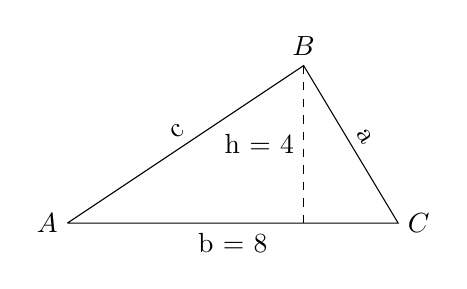
\begin{tikzpicture}[scale=1]
      \coordinate [label=left:$A$] (A) at (-2cm,-1.cm);
      \coordinate [label=right:$C$] (C) at (2.2cm,-1.0cm);
      \coordinate [label=above:$B$] (B) at (1cm,1.0cm);
      \draw (A) -- node[sloped,above] {c} (B) -- node[sloped,above,] {a} (C) -- node[below] {b = 8} (A);
      \draw[dashed] (B) -- node[left] {h = 4} (A-|B);
    \end{tikzpicture}
  \end{align*}
  \begin{align}
    b &= 8 \text{, the base of the triangle} \\
    h &= 4 \text{, the height of the triangle} \\
    A &= \frac{b \cdot h}{2} \text{, formula for the area of a triangle}
  \end{align}
  \item Write a program that calculates the area of a rectangle given the length and width.
  \begin{align*}
    \begin{tikzpicture}[scale=1]
      \coordinate [label=left:$A$] (A) at (-2cm,1cm);
      \coordinate [label=right:$B$] (B) at (2cm,1cm);
      \coordinate [label=right:$C$] (C) at (2cm,-1cm);
      \coordinate [label=left:$D$] (D) at (-2cm,-1cm);
      \draw (A) -- node[above] {w = 4} (B) -- node[right] {l = 2} (C) -- (D) -- (A);
    \end{tikzpicture}
  \end{align*}
  \begin{align}
    l &= 2 \text{, the length of the rectangle} \\
    w &= 4 \text{, the width of the rectangle} \\
    A &= l \cdot w \text{, formula for the area of a rectangle}
  \end{align}
  \item Write a program that calculates the area of a circle given the radius.
  \begin{align*}
    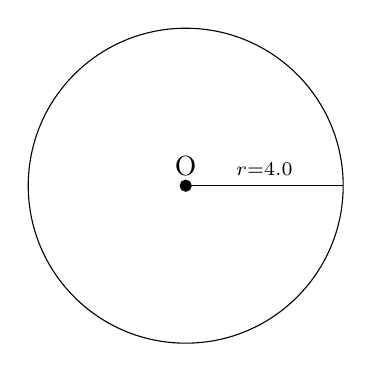
\begin{tikzpicture}[scale=1]
      \draw (2,2) circle (2cm);
      \draw[fill=black](2,2) circle (2 pt) node [above] {O};
      \draw[](2,2) -- (4,2) node [midway,above] {$\scriptstyle r = 4.0$};
    \end{tikzpicture}
  \end{align*}
  \begin{align}
    r &= 4.0 \text{, the radius of the circle} \\
    \pi &= 3.141592653589793 \text{, the mathematical constant pi} \\
    A &= \pi \cdot r^2 \text{, formula for the area of a circle}
  \end{align}
\end{enumerate}

\section{Data Types}

Data types specify the different sizes and values that can be stored in a variable.
There are two types of data types in Java:

\begin{itemize}
  \item \textnormal{Primitive Data Types: These data types are predefined by the language
  and are named by a reserved keyword. They are used to store simple values.}
  \item \textnormal{Non-Primitive Data Types: These data types are not predefined by the
  language and are created by the programmer. They are also known as reference types
  because they refer to objects.}
\end{itemize}

\subsection{Primitive Data Types}

Primitive data types are predefined by the language and are named by a reserved
keyword. They are used to store simple values. There are eight primitive data
types in Java:

\begin{table}[h!]
  \centering
  \caption{Primitive Data Types in Java}
  \begin{tabular*}{\hsize}{@{\extracolsep{\fill}}l l p{12cm} @{}}
      \toprule
      Data Type & Bytes & Description \\
      \colrule
      byte & 1 & Stores whole numbers from -128 to 127 \\
      short & 2 & Stores whole numbers from -32,768 to 32,767 \\
      int & 4 & Stores whole numbers from -2,147,483,648 to 2,147,483,647 \\
      long & 8 & Stores whole numbers from -9,223,372,036,854,775,808 to 9,223,372,036,854,775,807 \\
      float & 4 & Stores fractional numbers. Sufficient for storing 6 to 7 decimal digits \\
      double & 8 & Stores fractional numbers. Sufficient for storing 15 decimal digits \\
      char & 2 & Stores a single character/letter or ASCII values \\
      boolean & 1 & Stores true or false values \\
      \botrule
  \end{tabular*}
  \label{tab:primitive-data-types}
\end{table}

The table above shows the eight primitive data types in Java, along with their
sizes in bytes and descriptions.

\subsubsection{byte}

The ``byte'' data type is an 8-bit signed integer. It has a minimum value of -128
and a maximum value of 127 (inclusive). The ``byte'' data type is used to save
space in large arrays, mainly in place of integers, since a byte is four times
smaller than an int. 

\begin{lstlisting}[language=Java, caption={Byte Data Type}]
  byte byteVariable = 100;
\end{lstlisting}

\subsubsection{short}

The ``short'' data type is a 16-bit signed integer. It has a minimum value of
-32,768 and a maximum value of 32,767 (inclusive). The ``short'' data type is
used to save memory in large arrays, mainly in place of integers, since a short
is two times smaller than an int.

\begin{lstlisting}[language=Java, caption={Short Data Type}]
  short shortVariable = 1000;
\end{lstlisting}

\subsubsection{int}

The ``int'' data type is a 32-bit signed integer. It has a minimum value of
-2,147,483,648 and a maximum value of 2,147,483,647 (inclusive). The ``int''
data type is generally used as the default data type for integral values unless
there is a concern about memory.

\begin{lstlisting}[language=Java, caption={Int Data Type}]
  int intVariable = 100000;
\end{lstlisting}

\subsubsection{long}

The ``long'' data type is a 64-bit signed integer. It has a minimum value of
-9,223,372,036,854,775,808 and a maximum value of 9,223,372,036,854,775,807
(inclusive). The ``long'' data type is used when you need a range of values more
than those provided by int.

\begin{lstlisting}[language=Java, caption={Long Data Type}]
  long longVariable = 100000000L;
\end{lstlisting}

To indicate that a value is of the ``long'' data type, you must append an ``L''
to the value. The ``L'' tells the compiler that the value is a long literal. If
you do not append an ``L'' to the value, the compiler will treat it as an int
literal. This can lead to a compilation error if the value is too large to be
represented as an int.

\subsubsection{float}

The ``float'' data type is a single-precision 32-bit IEEE 754 floating-point. It
should never be used for precise values, such as currency. This is because it
will result in a loss of precision. The ``float'' data type is used when you need
a fractional value with a large range.

\begin{lstlisting}[language=Java, caption={Float Data Type}]
  float floatVariable = 234.5f;
\end{lstlisting}

To indicate that a value is of the ``float'' data type, you must append an ``f''
to the value. The ``f'' tells the compiler that the value is a float literal. If
you do not append an ``f'' to the value, the compiler will treat it as a double
literal.

\subsubsection{double}

The ``double'' data type is a double-precision 64-bit IEEE 754 floating-point. It
can store fractional values with a large range. The ``double'' data type is used
when you need a fractional value with a large range.

\begin{lstlisting}[language=Java, caption={Double Data Type}]
  double doubleVariable = 123.4;
\end{lstlisting}

Unlike the ``float'' data type, the ``double'' data type does not require any
appending characters to indicate that a value is of the ``double'' data type. The
compiler will treat any value with a decimal point as a double literal.

\subsubsection{char}

The ``char'' data type is a single 16-bit Unicode character. It has a minimum
value of \textnormal{\textbackslash{u0000}} (or 0) and a maximum value of
\textnormal{\textbackslash{u0041}} (or 65,535 inclusive).

\begin{lstlisting}[language=Java, caption={Char Data Type}]
  char charVariable = 'A';
\end{lstlisting}

When you assign a character literal to a char variable, you must enclose the
character in single quotes. Character literals are enclosed in single quotes,
such as 'A' or '7'. If you enclose a character in double quotes, it will be
treated as a string literal.

\begin{lstlisting}[language=Java, caption={Char Data Type using ASCII Value}]
  char charVariable = 65;
\end{lstlisting}

A number from 0 to 65535 can also be used to represent a character. For example,
65 represents the character 'A', and 97 represents the character 'a'. This is
because the ASCII value of 'A' is 65, and the ASCII value of 'a' is 97.

\begin{lstlisting}[language=Java, caption={Char Data Type using Unicode Escape}]
  char charVariable = '\u0041';
\end{lstlisting}

You can also use Unicode escape sequences to represent characters. For example,
'\u0041' represents the character 'A' in the Latin alphabet.

\subsubsection{boolean}

The ``boolean'' data type represents one bit of information, but its ``size'' isn't
precisely defined. It can only take the values true or false.

\begin{lstlisting}[language=Java, caption={Boolean Data Type}]
  boolean booleanVariable = true;
\end{lstlisting}

Aside from representing true or false, a boolean can also represent values
with two states, such as on or off, yes or no, or 0 or 1.

\subsection{Non-Primitive Data Types}

Non-primitive data types are not predefined by the language and are created by
the programmer. They are also known as reference types because they refer to
objects. There are two types of non-primitive data types:

\begin{itemize}
  \item \textnormal{Reference Data Types: Reference variables are created using defined
  classes. They are used to access objects.}
  \item \textnormal{Array Data Types: Array data types are used to store multiple values in
  a single variable.}
\end{itemize}

\subsubsection{Reference Data Types}

Reference variables are created using defined classes. They are used to access
objects.

\paragraph{String}

The ``String'' class represents a sequence of characters. Strings are immutable,
which means they cannot be changed after they are created.

\begin{lstlisting}[language=Java, caption={String Data Type}]
  String stringVariable = new String("Hello, World!");
\end{lstlisting}

\paragraph{ArrayList}

The ``ArrayList'' class is a resizable array that implements the List interface.
It allows you to add, remove, and access elements based on their index.

\begin{lstlisting}[language=Java, caption={ArrayList Data Type}]
  List<String> arrayListVariable = new ArrayList<String>();
  arrayListVariable.add("Apple");
  arrayListVariable.add("Banana");
\end{lstlisting}

\paragraph{HashMap}

The ``HashMap'' class is a hash table-based implementation of the Map interface.
It allows you to store key-value pairs and access the values based on their keys.

\begin{lstlisting}[language=Java, caption={HashMap Data Type}]
  Map<String, String> hashMapVariable = new HashMap<String, String>();
  hashMapVariable.put("Key1", "Value1");
  hashMapVariable.put("Key2", "Value2");
\end{lstlisting}

\paragraph{HashSet}

The ``HashSet'' class is an implementation of the Set interface. It stores unique
elements and does not allow duplicates.

\begin{lstlisting}[language=Java, caption={HashSet Data Type}]
  Set<String> hashSetVariable = new HashSet<String>();
  hashSetVariable.add("Apple");
  hashSetVariable.add("Banana");
\end{lstlisting}

\paragraph{LinkedList}

The ``LinkedList'' class is a doubly-linked list implementation of the List and
Deque interfaces. It allows you to add, remove, and access elements based on their
index.

\begin{lstlisting}[language=Java, caption={LinkedList Data Type}]
  List<String> linkedListVariable = new LinkedList<String>();
  linkedListVariable.add("Apple");
  linkedListVariable.add("Banana");
\end{lstlisting}

\paragraph{Queue}

The ``Queue'' interface represents a collection of elements that can be added or
removed in a specific order. The ``LinkedList'' class implements the Queue interface.

\begin{lstlisting}[language=Java, caption={Queue Data Type}]
  Queue<String> queueVariable = new LinkedList<String>();
  queueVariable.add("Apple");
  queueVariable.add("Banana");
\end{lstlisting}

\paragraph{Stack}

The ``Stack'' class represents a last-in, first-out (LIFO) stack of elements. It
extends the Vector class with five operations that allow a vector to be treated
as a stack.

\begin{lstlisting}[language=Java, caption={Stack Data Type}]
  Stack<String> stackVariable = new Stack<String>();
  stackVariable.push("Apple");
  stackVariable.push("Banana");
\end{lstlisting}

\paragraph{TreeMap}

The ``TreeMap'' class is a Red-Black tree-based implementation of the Map interface.
It provides an efficient means of storing key-value pairs in sorted order.

\begin{lstlisting}[language=Java, caption={TreeMap Data Type}]
  Map<String, String> treeMapVariable = new TreeMap<String, String>();
  treeMapVariable.put("Key1", "Value1");
  treeMapVariable.put("Key2", "Value2");
\end{lstlisting}

\paragraph{TreeSet}

The ``TreeSet'' class is an implementation of the Set interface. It stores unique
elements in sorted order.

\begin{lstlisting}[language=Java, caption={TreeSet Data Type}]
  Set<String> treeSetVariable = new TreeSet<String>();
  treeSetVariable.add("Apple");
  treeSetVariable.add("Banana");
\end{lstlisting}

\subsubsection{Array Data Types}

Array data types are used to store multiple values in a single variable. To
create an array, you must specify the data type of the elements and the size of
the array. To access an element in an array, you must use the index of the element.

\begin{lstlisting}[language=Java, caption={Array Data Types}]
  int[] intArrayVariable = new int[5];
  intArrayVariable[0] = 10;
  intArrayVariable[1] = 20;
  intArrayVariable[2] = 30;
  intArrayVariable[3] = 40;
  intArrayVariable[4] = 50;

  String[] stringArrayVariable = new String[2];
  stringArrayVariable[0] = "Hello";
  stringArrayVariable[1] = "World";

  System.out.print("Int Array: ");
  for (int i = 0; i < intArrayVariable.length; i++) {
    System.out.print(intArrayVariable[i] + " ");
  }
  System.out.println();

  System.out.print("String Array: ");
  for (int i = 0; i < stringArrayVariable.length; i++) {
    System.out.print(stringArrayVariable[i] + " ");
  }
  System.out.println();

  // Output
  // Int Array: 10 20 30 40 50
\end{lstlisting}

The code above demonstrates the use of array data types in Java. The code creates
two arrays, one for integers and one for strings. It assigns values to the elements
of the arrays and then prints the arrays to the console.

\subsection{Summary}

Data types specify the different sizes and values that can be stored in a variable.
There are two types of data types in Java: primitive data types and non-primitive
data types.

Primitive data types are predefined by the language and are used to store simple
values. There are eight primitive data types in Java: byte, short, int, long,
float, double, char, and boolean.

Non-primitive data types are not predefined by the language and are created by
the programmer. They are used to access objects and store multiple values in a
single variable. Non-primitive data types include reference data types and array
data types.

\subsection{Coding Exercises}

\begin{enumerate}
  \item \textnormal{Create a Java program that declares and initializes a variable
  of the following data types: byte, short, int, long, float, double, char,
  boolean, String, and an array of integers. Print the values of the variables to
  the console.}
\end{enumerate}

\section{Basic Object-Oriented Programming Concepts}

Object-Oriented Programming (OOP) is a programming paradigm that relies on the
concept of classes and objects. It is used to structure a software program into
simple, reusable pieces of code blueprints (usually called classes), which are
used to create individual instances of objects.

The main principles of OOP are:

\begin{itemize}
  \item \textnormal{Encapsulation: Encapsulation is the mechanism that binds
  together code and the data it manipulates, and keeps both safe from outside
  interference and misuse.}
  \item \textnormal{Inheritance: Inheritance is a mechanism in which one object
  acquires all the properties and behaviors of a parent object.}
  \item \textnormal{Polymorphism: Polymorphism is the ability of an object to
  take on many forms.}
  \item \textnormal{Abstraction: Abstraction is a concept of object-oriented
  programming that allows hiding the implementation details and showing only
  the functionality to the user.}
\end{itemize}

In Object-Oriented Programming (OOP), a class is a blueprint for creating objects.
A class provides initial values for state (member variables or attributes) and
implementations of behavior (member functions or methods). A class is a user-defined
data type that can be used in a program and works as an object constructor or a
blueprint for creating objects.

\begin{lstlisting}[language=Java, caption={Animal Class}]
  // Animal.java

  public class Animal {
      String name;
      String species;
      int age;
      int weight;
      String color;
      String habitat;

      int x;
      int y;

      public Animal(String name, String species, int age, int weight, String color, String habitat, int x, int y) {
          this.name = name;
          this.species = species;
          this.age = age;
          this.weight = weight;
          this.color = color;
          this.habitat = habitat;
          this.x = x;
          this.y = y;
      }

      void makeSound() {
          System.out.println(this.name + " makes a sound.");
      }

      void move(int x, int y) {
          this.x = x;
          this.y = y;
          System.out.println("The animal moves to (" + x + ", " + y + ").");
      }

      void eat() {
          System.out.println("The animal eats food.");
      }

      void sleep() {
          System.out.println("The animal sleeps.");
      }
  }
\end{lstlisting}

The ``Animal'' class is a blueprint for creating objects of type ``Animal''. It
provides initial values for state (member variables or attributes) and implementations
of behavior (member functions or methods).

The syntax for creating a class in Java is:

\begin{lstlisting}[language=Java, caption={Class Syntax}]
  public class ClassName {
      // member variables or attributes
      // member functions or methods
  }
\end{lstlisting}

\begin{lstlisting}[language=Java, caption={Class Attributes}]
  public class Animal {
      String name;
      String species;
      int age;
      int weight;
      String color;
      String habitat;
      int x;
      int y;

      // Rest of the code...
  }
\end{lstlisting}

The ``Animal'' class has member variables or attributes that represent the state
of an animal, such as its name, species, age, weight, color, habitat, and position
(x, y). These attributes represents the real-world properties of an animal.

% Constructor
\begin{lstlisting}[language=Java, caption={Class Constructor}]
  public class Animal {
      // Member variables or attributes...

      public Animal(String name, String species, int age, int weight, String color, String habitat, int x, int y) {
          this.name = name;
          this.species = species;
          this.age = age;
          this.weight = weight;
          this.color = color;
          this.habitat = habitat;
          this.x = x;
          this.y = y;
      }
      
      // Rest of the code...
  }
\end{lstlisting}

A constructor is a special method that is used to initialize objects. It is called
when an object of a class is created. It has the same name as the class and does
not have a return type. Constructors are used to set initial values for the member
variables of an object.

% Methods

\begin{lstlisting}[language=Java, caption={Class Methods}]
  public class Animal {
      // Member variables or attributes...
      
      // Constructor...
      
      void makeSound() {
          System.out.println(this.name + " makes a sound.");
      }

      void move(int x, int y) {
          this.x = x;
          this.y = y;
          System.out.println("The animal moves to (" + x + ", " + y + ").");
      }

      void eat() {
          System.out.println("The animal eats food.");
      }

      void sleep() {
          System.out.println("The animal sleeps.");
      }
  }
\end{lstlisting}

The ``Animal'' class has member functions or methods that represent the behavior
of an animal, such as making a sound, moving to a new position, eating food, and
sleeping. These methods represent the actions that an animal can perform.

\subsection{Why use Object-Oriented Programming?}

Object-oriented programming (OOP) has several advantages over procedural programming.
Some of the key benefits of OOP are:

\begin{itemize}
  \item \textbf{Modularity:} OOP programs are divided into objects, which can be
  developed independently. This makes the code more modular, reusable, and easier
  to maintain.
  \item \textbf{Code Reusability:} OOP promotes code reusability through inheritance
  and polymorphism. Classes can be reused in different parts of the program without
  modification.
  \item \textbf{Encapsulation:} OOP encapsulates the data and methods within a class,
  which protects the data from being accessed or modified by unauthorized code.
  \item \textbf{Abstraction:} OOP provides abstraction by hiding the implementation
  details and showing only the functionality to the user. This simplifies the
  complexity of the program.
  \item \textbf{Inheritance:} OOP allows classes to inherit the properties and methods
  of other classes, which promotes code reusability and reduces the complexity of
  the program.
  \item \textbf{Polymorphism:} OOP allows methods to do different things based on
  the object that they are acting upon. This provides flexibility and code reusability.
\end{itemize}

OOP is widely used in software development because of its ability to model real-world
entities, promote code reusability, and simplify the complexity of the program.
It is a powerful paradigm that helps in developing scalable, maintainable, and
flexible software applications.

\subsection{Inheritance}

Inheritance is a mechanism in which one object acquires all the properties and
behaviors of a parent object. It allows a class to inherit the properties and
methods of another class. The class which inherits the properties and methods is
known as the child class, and the class whose properties and methods are inherited
is known as the parent class. Inheritance is an important feature of OOP that
allows code reusability and reduces the complexity of a program.

\begin{lstlisting}[language=Java, caption={Mammal Class (Inheritance)}]
  // Mammal.java

  public class Mammal extends Animal {
      String fur;
      boolean milk;
      boolean isWarmBlooded;
      boolean canGiveBirth;

      Mammal(String name, String species, int age, int weight, String color, String habitat, int x, int y) {
          super(name, species, age, weight, color, habitat, x, y);
      }

      Mammal(String name, String species, int age, int weight, String color, String habitat, int x, int y, String fur, boolean milk, boolean isWarmBlooded, boolean canGiveBirth) {
          super(name, species, age, weight, color, habitat, x, y);
          this.fur = fur;
          this.milk = milk;
          this.isWarmBlooded = isWarmBlooded;
          this.canGiveBirth = canGiveBirth;
      }

      void giveBirth() {
          if (this.age >= 2 && this.canGiveBirth) {
              System.out.println(this.name + " is giving birth.");
          } else {
              System.out.println(this.name + " is too young to give birth.");
          }
      }
  }
\end{lstlisting}

The ``Mammal'' class is a child class of the ``Animal'' class. It inherits the
properties and methods of the ``Animal'' class.

% Member Variables

\begin{lstlisting}[language=Java, caption={Mammal Class (Member Variables)}]
  public class Mammal extends Animal {
      String fur;
      boolean milk;
      boolean isWarmBlooded;
      boolean canGiveBirth;

      // Rest of the code...
  }
\end{lstlisting}

The ``Mammal'' class has member variables or attributes that represent the state
of a mammal, such as its fur, milk production, warm-blooded nature, and ability
to give birth. These attributes represent the real-world properties of a mammal.

% Constructors

\begin{lstlisting}[language=Java, caption={Mammal Class (Constructors)}]
  public class Mammal extends Animal {
      // Member variables or attributes...

      Mammal(String name, String species, int age, int weight, String color, String habitat, int x, int y) {
          super(name, species, age, weight, color, habitat, x, y);
      }

      Mammal(String name, String species, int age, int weight, String color, String habitat, int x, int y, String fur, boolean milk, boolean isWarmBlooded, boolean canGiveBirth) {
          super(name, species, age, weight, color, habitat, x, y);
          this.fur = fur;
          this.milk = milk;
          this.isWarmBlooded = isWarmBlooded;
          this.canGiveBirth = canGiveBirth;
      }

      // Rest of the code...
  }
\end{lstlisting}

The ``Mammal'' class has two constructors that initialize the member variables of
the ``Mammal'' class as well as the ``Animal'' class. Having multiple constructors
in a class is called method overloading.

% First Constructor

\begin{lstlisting}[language=Java, caption={Mammal Class (First Constructor)}]
  Mammal(String name, String species, int age, int weight, String color, String habitat, int x, int y) {
      super(name, species, age, weight, color, habitat, x, y);
  }
\end{lstlisting}

The first constructor initializes the member variables of the ``Mammal'' class.
This constructor calls the constructor of the parent class (``Animal'') using the
``super'' keyword.

% Second Constructor

\begin{lstlisting}[language=Java, caption={Mammal Class (Second Constructor)}]
  Mammal(String name, String species, int age, int weight, String color, String habitat, int x, int y, String fur, boolean milk, boolean isWarmBlooded, boolean canGiveBirth) {
      super(name, species, age, weight, color, habitat, x, y);
      this.fur = fur;
      this.milk = milk;
      this.isWarmBlooded = isWarmBlooded;
      this.canGiveBirth = canGiveBirth;
  }
\end{lstlisting}

The second constructor initializes the member variables of the ``Mammal'' class as
well as the ``Animal'' class. This constructor allows additional properties of a
mammal to be set, such as fur, milk production, warm-blooded nature, and ability
to give birth.

% Methods

\begin{lstlisting}[language=Java, caption={Mammal Class (Methods)}]
  public class Mammal extends Animal {
      // Member variables or attributes...
      
      // Constructors...

      void giveBirth() {
          if (this.age >= 2 && this.canGiveBirth) {
              System.out.println(this.name + " is giving birth.");
          } else {
              System.out.println(this.name + " is too young to give birth.");
          }
      }
  }
\end{lstlisting}

The ``Mammal'' class has a method called ``giveBirth()'' that makes the mammal
give birth. This method is specific to the ``Mammal'' class and is not present
in the ``Animal'' class.

\subsection{Encapsulation}

Encapsulation is the mechanism that binds together code and the data it manipulates,
and keeps both safe from outside interference and misuse. One way to think about
encapsulation is as a protective wrapper that prevents the code and data from being
arbitrarily accessed by other code defined outside the wrapper.

Encapsulation is used to:

\begin{itemize}
  \item \textnormal{Control the way data is accessed or modified}
  \item \textnormal{Prevent data from being modified by unauthorized code}
  \item \textnormal{Allow data to be accessed only through getter methods}
  \item \textnormal{Protect the integrity of the data}
\end{itemize}

Encapsulation is an important concept in OOP that helps in maintaining the integrity
of the data and the code that manipulates it.

\begin{lstlisting}[language=Java, caption={Dog Class(Encapsulation)}]
  // Dog.java

  public class Dog extends Mammal {
      private String breed;
      private String barkingSound;
      private boolean tailWagging;
      private boolean isTrained;

      Dog(String name, String species, int age, int weight, String color, String habitat, int x, int y, String fur, boolean milk, boolean isWarmBlooded, boolean canGiveBirth, String breed, String barkingSound, boolean tailWagging, boolean isTrained) {
          super(name, species, age, weight, color, habitat, x, y, fur, milk, isWarmBlooded, canGiveBirth);
          this.breed = breed;
          this.barkingSound = barkingSound;
          this.tailWagging = tailWagging;
          this.isTrained = isTrained;
      }

      public String getBreed() {
          return breed;
      }

      public void setBreed(String breed) {
          this.breed = breed;
      }

      public String getBarkingSound() {
          return barkingSound;
      }

      public void setBarkingSound(String barkingSound) {
          this.barkingSound = barkingSound;
      }

      public boolean isTailWagging() {
          return tailWagging;
      }

      public void setTailWagging(boolean tailWagging) {
          this.tailWagging = tailWagging;
      }

      public boolean isTrained() {
          return isTrained;
      }

      public void setTrained(boolean isTrained) {
          this.isTrained = isTrained;
      }

      public void bark() {
          System.out.println("The dog barks: " + barkingSound);
      }

      public void fetch() {
          if (this.isTrained) {
              System.out.println("The dog fetches the ball.");
          } else {
              System.out.println("The dog is not trained to fetch.");
          }
      }

      public void wagTail() {
          if (this.tailWagging) {
              System.out.println("The dog wags its tail.");
          } else {
              System.out.println("The dog is not wagging its tail.");
          }
      }

      public void sit() {
          if (this.isTrained) {
              System.out.println("The dog sits.");
          } else {
              System.out.println("The dog is not trained to sit.");
          }
      }
  }
\end{lstlisting}

The ``Dog'' class is a child class of the ``Mammal'' class. It inherits the properties
and methods of the ``Mammal'' class. The ``Dog'' class also inherits the ``Animal''
class through the ``Mammal'' class. The ``Dog'' class demonstrates the concept of
encapsulation by using private member variables and providing public getter and
setter methods to access and modify the private member variables.

% Getter and Setter Methods

\begin{lstlisting}[language=Java, caption={Dog Class (Getter and Setter Methods)}]
  public class Dog extends Mammal {
      // Member variables or attributes...
      
      // Constructor...

      public String getBreed() {
          return breed;
      }

      public void setBreed(String breed) {
          this.breed = breed;
      }

      public String getBarkingSound() {
          return barkingSound;
      }

      public void setBarkingSound(String barkingSound) {
          this.barkingSound = barkingSound;
      }

      public boolean isTailWagging() {
          return tailWagging;
      }

      public void setTailWagging(boolean tailWagging) {
          this.tailWagging = tailWagging;
      }

      public boolean isTrained() {
          return isTrained;
      }

      public void setTrained(boolean isTrained) {
          this.isTrained = isTrained;
      }

      // Rest of the code...
  }
\end{lstlisting}

The ``Dog'' class has private member variables that represent the state of a dog,
such as its breed, barking sound, tail-wagging behavior, and training status. These
member variables are private to the class, which means they cannot be accessed or
modified directly from outside the class. To access or modify these private member
variables, the ``Dog'' class provides public getter and setter methods.

% Getter Methods

\begin{lstlisting}[language=Java, caption={Dog Class (Getter Methods)}]
  public String getBreed() {
      return breed;
  }

  public String getBarkingSound() {
      return barkingSound;
  }

  public boolean isTailWagging() {
      return tailWagging;
  }

  public boolean isTrained() {
      return isTrained;
  }
\end{lstlisting}

The getter methods are used to access the value of a private member variable. They
return the value of the private member variable to the caller. The getter methods
are public, which means they can be accessed from outside the class. They provide
read-only access to the private member variables. For convention, the getter methods
are named with the prefix ``get'' followed by the name of the member variable.

Aside for its read-only access, the getter methods are also used to perform additional
operations, such as validation or computation, before returning the value of the
private member variable. This allows the class to maintain the integrity of the
data and provide a consistent interface to the caller.

% Setter Methods

\begin{lstlisting}[language=Java, caption={Dog Class (Setter Methods)}]
  public void setBreed(String breed) {
      this.breed = breed;
  }

  public void setBarkingSound(String barkingSound) {
      this.barkingSound = barkingSound;
  }

  public void setTailWagging(boolean tailWagging) {
      this.tailWagging = tailWagging;
  }

  public void setTrained(boolean isTrained) {
      this.isTrained = isTrained;
  }
\end{lstlisting}

The setter methods are used to set the value of a private member variable. They
assign a new value to the private member variable based on the input provided by
the caller. The setter methods are public, which means they can be accessed from
outside the class. They provide write-only access to the private member variables.
For convention, the setter methods are named with the prefix ``set'' followed by
the name of the member variable.

Aside for its write-only access, the setter methods are also used to perform additional
operations, such as validation or computation, before setting the value of the private
member variable. For example, in a website where users have different roles, the
setter method can be used to check if the user has the necessary permissions to
set the value of a private member variable.

\subsection{Polymorphism}

Polymorphism is the ability of an object to take on many forms. The most common
use of polymorphism in OOP occurs when a parent class reference is used to refer
to a child class object. Polymorphism allows methods to do different things based
on the object that they are acting upon. It is a powerful feature of OOP that
allows code reusability and flexibility.

\begin{lstlisting}[language=Java, caption={Bird Class (Polymorphism)}]
  // Bird.java

  public class Bird extends Animal {
      private int wings;
      private boolean hasFeathers;
      private boolean canFly;
      private boolean canLayEggs;

      Bird(String name, String species, int age, int weight, String color, String habitat, int x, int y, int wings, boolean hasFeathers, boolean canFly, boolean canLayEggs) {
          super(name, species, age, weight, color, habitat, x, y);
          this.wings = wings;
          this.hasFeathers = hasFeathers;
          this.canFly = canFly;
          this.canLayEggs = canLayEggs;
      }

      public int getWings() {
          return wings;
      }

      public void setWings(int wings) {
          this.wings = wings;
      }

      public boolean isHasFeathers() {
          return hasFeathers;
      }

      public void setHasFeathers(boolean hasFeathers) {
          this.hasFeathers = hasFeathers;
      }

      public boolean canFly() {
          return canFly;
      }

      public void setCanFly(boolean canFly) {
          this.canFly = canFly;
      }

      public boolean canLayEggs() {
          return canLayEggs;
      }

      public void setCanLayEggs(boolean canLayEggs) {
          this.canLayEggs = canLayEggs;
      }

      public void fly() {
          if (canFly && hasFeathers) {
              System.out.println(name + " is flying.");
          } else {
              System.out.println(name + " cannot fly.");
          }
      }

      public void layEggs() {
          if (this.age >= 1 && canLayEggs) {
              System.out.println(name + " is laying eggs.");
          } else {
              System.out.println(name + " is too young to lay eggs.");
          }
      }

      @Override
      void makeSound() {
          System.out.println(this.name + " chirps.");
      }
  }
\end{lstlisting}

The ``Bird'' class is a child class of the ``Animal'' class. It inherits the
properties and methods of the ``Animal'' class. The ``Bird'' class demonstrates
the concept of polymorphism by overriding the ``makeSound()'' method of the
``Animal'' class.

% Overriding Methods

\begin{lstlisting}[language=Java, caption={Bird Class (Overriding Methods)}]
  @Override
  void makeSound() {
      System.out.println(this.name + " chirps.");
  }
\end{lstlisting}

The ``Bird'' class overrides the ``makeSound()'' method of the ``Animal'' class.
The ``makeSound()'' method makes the bird chirp. This method is specific to the
``Bird'' class and is not present in the ``Animal'' class.

% makeSound() Method in Animal Class

\begin{lstlisting}[language=Java, caption={Animal Class (makeSound() Method)}]
  // Animal.java (makeSound() method)
  void makeSound() {
      System.out.println(this.name + " makes a sound.");
  }
\end{lstlisting}

For objects of the ``Bird'' class, the ``makeSound()'' method will output ``chirps''
instead of the default ``makes a sound'' output of the ``Animal'' class. This is
an example of polymorphism in action, where the same method name is used in both
the parent and child classes, but the behavior of the method is different based
on the object that it is acting upon.

\subsection{Abstraction}

Abstraction is a concept of object-oriented programming that allows hiding the
implementation details and showing only the functionality to the user. It helps
to reduce programming complexity and effort.

An abstract class is a class that cannot be instantiated. It is used to provide
a common interface for all the classes that inherit from it. Abstract classes can
have abstract methods that are declared but not implemented. These methods must
be implemented by the child classes that inherit from the abstract class.

\begin{lstlisting}[language=Java, caption={Reptile Class (Abstraction)}]
  // Reptile.java

  public abstract class Reptile extends Animal {
      private boolean hasScales;
      private boolean hasTail;
      private boolean isColdBlooded;
      private boolean canRegenerateTail;
      private boolean canLayEggs;

      Reptile(String name, String species, int age, int weight, String color, String habitat, int x, int y, boolean hasScales, boolean hasTail, boolean isColdBlooded, boolean canRegenerateTail, boolean canLayEggs) {
          super(name, species, age, weight, color, habitat, x, y);
          this.hasScales = hasScales;
          this.hasTail = hasTail;
          this.isColdBlooded = isColdBlooded;
          this.canRegenerateTail = canRegenerateTail;
          this.canLayEggs = canLayEggs;
      }

      public abstract void biteHuman();

      public boolean hasScales() {
          return hasScales;
      }

      public void setHasScales(boolean hasScales) {
          this.hasScales = hasScales;
      }

      public boolean isColdBlooded() {
          return isColdBlooded;
      }

      public void setColdBlooded(boolean isColdBlooded) {
          this.isColdBlooded = isColdBlooded;
      }

      public boolean canRegenerateTail() {
          return canRegenerateTail;
      }

      public void setCanRegenerateTail(boolean canRegenerateTail) {
          this.canRegenerateTail = canRegenerateTail;
      }

      public boolean canLayEggs() {
          return canLayEggs;
      }

      public void setCanLayEggs(boolean canLayEggs) {
          this.canLayEggs = canLayEggs;
      }

      public void shedSkin() {
          if (hasScales) {
              System.out.println(name + " is shedding its skin.");
          } else {
              System.out.println(name + " does not have scales and cannot shed its skin.");
          }
      }

      public void layEggs() {
          if (canLayEggs) {
              System.out.println(name + " is laying eggs.");
          } else {
              System.out.println(name + " cannot lay eggs.");
          }
      }

      public void regenerateTail() {
          if (canRegenerateTail && hasTail) {
              System.out.println(name + " is regenerating its tail.");
          } else {
              System.out.println(name + " cannot regenerate its tail.");
          }
      }
  }
\end{lstlisting}

The ``Reptile'' class is an abstract class that extends the ``Animal'' class. It
inherits the properties and methods of the ``Animal'' class and adds additional
properties and methods specific to reptiles. Since the ``Reptile'' class is an
abstract class, it cannot be instantiated.

\begin{lstlisting}[language=Java, caption={Reptile Class (Abstract Method)}]
  public abstract class Reptile extends Animal {
      // Member variables or attributes...
      
      // Constructor...

      public abstract void biteHuman();

      // Getter and setter methods...

      // Methods...
  }
\end{lstlisting}

The ``Reptile'' class has an abstract method called ``biteHuman()'' that must be
implemented by the child classes that inherit from the ``Reptile'' class. Abstract
methods are declared without an implementation and must be implemented by the child
classes.

The ``Snake'' class is a child class of the ``Reptile'' class which is an abstract
class. The ``Snake'' class inherits the properties and methods of the ``Reptile''
class and implements the abstract method ``biteHuman()''.

% Implementing Abstract Method

\begin{lstlisting}[language=Java, caption={Snake Class (Implementing Abstract Method)}]
  // Snake.java

  public class Snake extends Reptile {
      // Member variables or attributes...

      // Constructor...
      
      public void biteHuman() {
          System.out.println("The snake bites the human...");
          if (isVenomous) {
              System.out.println("The human is poisoned!");
          } else {
              System.out.println("The human is not poisoned.");
          }
      }

      // Getter and setter methods...

      // Methods...
  }
\end{lstlisting}

The ``Snake'' class implements the abstract method ``biteHuman()'' declared in
the ``Reptile'' class. The ``biteHuman()'' method simulates the snake biting a
human and poisoning the human if the snake is venomous.

\subsection{Using Classes and Objects}

Using the classes and objects defined in the previous sections, we can create
instances of the classes and interact with them.

\begin{lstlisting}[language=Java, caption={Basic Usage of Classes and Objects}]
  // BasicOOP.java

  public class BasicOOP {

      public static void main(String[] args) {
          Animal animal = new Animal("Dog", "Canis lupus familiaris", 5, 20, "Brown", "Domestic", 0, 0);

          System.out.println("Name: " + animal.name);
          System.out.println("Species: " + animal.species);
          System.out.println("Age: " + animal.age);

          animal.move(5, 10);

          Mammal mammal = new Mammal("Cat", "Felis catus", 3, 10, "White", "Domestic", 0, 0, "Short", true, true, true);
          Bird bird = new Bird("Eagle", "Aquila chrysaetos", 10, 15, "Brown", "Wild", 0, 0, 2, true, true, true);

          System.out.println("Mammal Name: " + mammal.name);
          System.out.println("Mammal Species: " + mammal.species);
          System.out.println("Mammal Age: " + mammal.age);

          System.out.println("Bird Name: " + bird.name);
          System.out.println("Bird Species: " + bird.species);
          System.out.println("Bird Age: " + bird.age);

          mammal.makeSound();
          bird.makeSound();

          Dog dog = new Dog("Buddy", "Golden Retriever", 2, 30, "Golden", "Domestic", 0, 0, "Golden", true, true, true, "Golden Retriever", "Woof!", true, true);

          System.out.println("Dog Name: " + dog.name);
          System.out.println("Dog Species: " + dog.species);
          System.out.println("Dog Age: " + dog.age);

          System.out.println("Bark sound when playing: " + dog.getBarkingSound());
          dog.setBarkingSound("Woof woof woof!");
          System.out.println("Bark sound when angry: " + dog.getBarkingSound());

          Snake snake = new Snake("Cobra", "Naja naja", 5, 10, "Black", "Wild", 0, 0, true, true, true, true, true, true, true);

          System.out.println("Snake Name: " + snake.name);
          System.out.println("Snake Species: " + snake.species);
          System.out.println("Snake Age: " + snake.age);

          snake.biteHuman();
      }
  }
\end{lstlisting}

The ``BasicOOP'' class demonstrates the use of classes and objects in Java to
implement OOP concepts such as inheritance, polymorphism, encapsulation, and
abstraction. It creates instances of the ``Animal'', ``Mammal'', ``Bird'',
``Dog'', and ``Snake'' classes and interacts with them by calling their methods
and accessing their properties.

\subsubsection{Object Creation and Initialization}

\begin{lstlisting}[language=Java, caption={Object Declaration and Initialization}]
  Animal animal = new Animal("Dog", "Canis lupus familiaris", 5, 20, "Brown", "Domestic", 0, 0);

  System.out.println("Name: " + animal.name);
  System.out.println("Species: " + animal.species);
  System.out.println("Age: " + animal.age);

  animal.move(5, 10);
\end{lstlisting}

In this code, we create an instance of the ``Animal'' class and initialize it with
some values. An ``object'' is an instance of a class. Declaring a variable of a
class is called ``declaration'', and assigning a value to the variable is called
``initialization''. When a class is defined, no memory is allocated, but when it
is instantiated (i.e., an object is created), memory is allocated. Instantiation is
the process of creating an object from a class. To access the properties and
methods of an object, we use the dot operator (``.''). For example, to access the
``name'' property of the ``animal'' object, we use ``animal.name''.

The syntax for creating an object in Java is:

\begin{lstlisting}[language=Java, caption={Object Creation Syntax}]
  ClassName objectName = new ClassName();
\end{lstlisting}

\subsubsection{Inheritance}

\begin{lstlisting}[language=Java, caption={Basic Inheritance}]
  Mammal mammal = new Mammal("Cat", "Felis catus", 3, 10, "White", "Domestic", 0, 0, "Short", true, true, true);
  Bird bird = new Bird("Eagle", "Aquila chrysaetos", 10, 15, "Brown", "Wild", 0, 0, 2, true, true, true);

  System.out.println("Mammal Name: " + mammal.name);
  System.out.println("Mammal Species: " + mammal.species);
  System.out.println("Mammal Age: " + mammal.age);

  System.out.println("Bird Name: " + bird.name);
  System.out.println("Bird Species: " + bird.species);
  System.out.println("Bird Age: " + bird.age);
\end{lstlisting}

In this code, we demonstrate inheritance by creating objects of the ``Mammal'' and
``Bird'' classes, which inherit from the ``Animal'' class. The ``Mammal'' and ``Bird''
classes inherit the properties and methods of the ``Animal'' class. We create
instances of the ``Mammal'' and ``Bird'' classes and access their properties such
as ``name'', ``species'', and ``age''.

\subsubsection{Polymorphism}

\begin{lstlisting}[language=Java, caption={Basic Polymorphism}]
  mammal.makeSound();
  bird.makeSound();
\end{lstlisting}

In this code, we demonstrate polymorphism by calling the ``makeSound()'' method on
the ``mammal'' and ``bird'' objects. The ``makeSound()'' method is defined in the
``Animal'' class and overridden in the ``Mammal'' and ``Bird'' classes. When the
``makeSound()'' method is called on the ``mammal'' and ``bird'' objects, the
implementation of the method in the respective classes is executed. This allows
the same method name to do different things based on the object that it is acting
upon.

\subsubsection{Encapsulation}

\begin{lstlisting}[language=Java, caption={Basic Encapsulation}]
  Dog dog = new Dog("Buddy", "Golden Retriever", 2, 30, "Golden", "Domestic", 0, 0, "Golden", true, true, true, "Golden Retriever", "Woof!", true, true);

  System.out.println("Dog Name: " + dog.name);
  System.out.println("Dog Species: " + dog.species);
  System.out.println("Dog Age: " + dog.age);

  System.out.println("Bark sound when playing: " + dog.getBarkingSound());
  dog.setBarkingSound("Woof woof woof!");
  System.out.println("Bark sound when angry: " + dog.getBarkingSound());
\end{lstlisting}

In this code, we demonstrate encapsulation by creating an instance of the ``Dog''
class and accessing the private member variables of the class using public getter
and setter methods. The ``Dog'' class has private member variables such as ``breed'',
``barkingSound'', ``tailWagging'', and ``isTrained''. We use the public getter
and setter methods to access and modify these private member variables. This
protects the data from being arbitrarily accessed or modified by other code defined
outside the class.

\subsubsection{Abstraction}

\begin{lstlisting}[language=Java, caption={Basic Abstraction}]
  /**
   * Trying to create an instance of the abstract class `Reptile` will result in
   * a compilation error.
   */
  // Reptile reptile = new Reptile("Lizard", "Lacertilia", 1, 1, "Green",
	// "Domestic", 0, 0, true, true, true, true,
	// true);

  Snake snake = new Snake("Cobra", "Naja naja", 5, 10, "Black", "Wild", 0, 0, true, true, true, true, true, true, true);

  System.out.println("Snake Name: " + snake.name);
  System.out.println("Snake Species: " + snake.species);
  System.out.println("Snake Age: " + snake.age);

  snake.biteHuman();
\end{lstlisting}

In this code, we demonstrate abstraction by creating an abstract class ``Reptile''
with abstract methods and creating a concrete class ``Snake'' that extends the
``Reptile'' class and implements the abstract methods. An abstract class cannot
be instantiated, but it can be used as a blueprint for other classes that inherit
from it. The ``Snake'' class extends the ``Reptile'' class and implements the
``biteHuman()'' method, which is declared as an abstract method in the ``Reptile''
class. The ``Snake'' class provides an implementation for the ``biteHuman()'' method,
which simulates the snake biting a human.

\subsection{Summary}

Object-oriented programming (OOP) is a programming paradigm that relies on the
concept of classes and objects. It is used to structure a software program into
simple, reusable pieces of code blueprints (usually called classes), which are
used to create individual instances of objects.

The main principles of OOP are:

\begin{itemize}
  \item Encapsulation is the mechanism that binds together code and the data it
  manipulates, and keeps both safe from outside interference and misuse.
  \item Inheritance is a mechanism in which one object acquires all the properties
  and behaviors of a parent object. It allows a class to inherit the properties
  and methods of another class.
  \item Polymorphism is the ability of an object to take on many forms. The most
  common use of polymorphism in OOP occurs when a parent class reference is used
  to refer to a child class object.
  \item Abstraction is a concept of object-oriented programming that allows hiding
  the implementation details and showing only the functionality to the user. It
  helps to reduce programming complexity and effort.
\end{itemize}

In Java, everything is an object aside from the primitive data types (e.g., int,
float, char, etc.). Java is an object-oriented programming language that is simple,
easy to learn, secure, robust, high performance, multithreaded, interpreted,
distributed, and dynamic.

%%%%%%%%%%%%%%%%%%%%%%%
%%%     Chapter     %%%
%%%%%%%%%%%%%%%%%%%%%%%
\chapter{Control Statements}

\section{Introduction}

Control statements are used to control the flow of execution in a program. They
allow you to make decisions, repeat code, and jump to different parts of the
program. Control statements are essential for writing programs that perform
different actions based on different conditions.

In Java, control statements can be categorized into the following types:

\begin{itemize}
  \item Conditional statements: These statements allow you to make decisions
  based on conditions. The most common conditional statements are the ``if'',
  ``if-else'', ``if-else-if ladder'', and ``switch'' statements.
  \item Iteration statements: These statements allow you to repeat a block of
  code multiple times. The most common iteration statements are the ``while'',
  ``do-while'', ``for'', and ``for-each'' loops.
  \item Jump statements: These statements allow you to jump to different parts
  of the program. The most common jump statements are the ``break'',
  ``continue'', and ``return'' statements.
\end{itemize}

\section{Conditional Statements and Decision Making}

Conditional statements are used to make decisions in a program. They allow you
to execute different blocks of code based on different conditions. Conditional
statements are essential for writing programs that perform different actions
based on different conditions.

\subsection{If Statement}

The ``if'' statement is used to execute a block of code if a specified condition
is true. If the condition is false, the code block is not executed.

\begin{lstlisting}[language=Java, caption={If Statement}]
  int x = 10;

  if (x > 0) {
      System.out.println("The number is positive.");
  }
\end{lstlisting}

In this code, the ``if'' statement checks if the value of the variable ``x'' is
greater than 0. If the condition is true, the message ``The number is positive.''
is printed to the console.

\subsection{If-Else Statement}

The ``if-else'' statement is used to execute a block of code if a specified
condition is true and another block of code if the condition is false.

\begin{lstlisting}[language=Java, caption={If-Else Statement}]
  int x = -5;

  if (x > 0) {
      System.out.println("The number is positive.");
  } else {
      System.out.println("The number is not positive.");
  }
\end{lstlisting}

In this code, the ``if-else'' statement checks if the value of the variable ``x''
is greater than 0. If the condition is true, the message ``The number is positive.''
is printed to the console. If the condition is false, the message ``The number is
not positive.'' is printed to the console.

\subsection{If-Else-If Ladder}

The ``if-else-if'' ladder is used to execute one block of code out of several
blocks based on multiple conditions. If the first condition is true, the first
block of code is executed. If the first condition is false and the second
condition is true, the second block of code is executed, and so on.

\begin{lstlisting}[language=Java, caption={If-Else-If Ladder}]
  int x = 0;

  if (x > 0) {
      System.out.println("The number is positive.");
  } else if (x < 0) {
      System.out.println("The number is negative.");
  } else {
      System.out.println("The number is zero.");
  }
\end{lstlisting}

In this code, the ``if-else-if'' ladder checks if the value of the variable ``x''
is greater than 0, less than 0, or equal to 0. Depending on the value of ``x'',
the corresponding message is printed to the console.

\subsection{Nested If-Else Statements}

Nested ``if-else'' statements are used to check multiple conditions within
another condition. The inner ``if-else'' statement is executed only if the
outer condition is true.

\begin{lstlisting}[language=Java, caption={Nested If-Else Statements}]
  int x = 10;
  int y = 20;

  if (x > 0) {
      if (y > 0) {
          System.out.println("Both numbers are positive.");
      } else {
          System.out.println("The first number is positive, but the second number is not positive.");
      }
  } else {
      System.out.println("The first number is not positive.");
  }
\end{lstlisting}

In this code, the outer ``if'' statement checks if the value of the variable ``x''
is greater than 0. If the condition is true, the inner ``if'' statement checks
if the value of the variable ``y'' is greater than 0. Depending on the values of
``x'' and ``y'', the corresponding message is printed to the console. If the
condition of the outer ``if'' statement is false, the message ``The first number
is not positive.'' is printed to the console.

\subsection{Switch Statement}

The ``switch'' statement is used to execute one block of code out of multiple
blocks based on the value of an expression. It is an alternative to the
``if-else-if'' ladder when you have to check multiple conditions based on the
value of a single expression. The ``switch'' statement is more efficient than
the ``if-else-if'' ladder when you have a large number of conditions to check.

\begin{lstlisting}[language=Java, caption={Switch Statement}]
  int day = 3;
  String dayName = "";

  switch (day) {
      case 1:
          dayName = "Monday";
          break;
      case 2:
          dayName = "Tuesday";
          break;
      case 3:
          dayName = "Wednesday";
          break;
      case 4:
          dayName = "Thursday";
          break;
      case 5:
          dayName = "Friday";
          break;
      case 6:
          dayName = "Saturday";
          break;
      case 7:
          dayName = "Sunday";
          break;
      default:
          dayName = "Invalid day";
          break;
  }

  System.out.println("The day is " + dayName);
\end{lstlisting}

In this code, the ``switch'' statement checks the value of the variable ``day''.
Depending on the value of ``day'', the corresponding day name is assigned to
the variable ``dayName''. If the value of ``day'' does not match any of the
``case'' values, the ``default'' block of code is executed.

\section{Iteration Statements}

Iteration statements are used to repeat a block of code multiple times. They
allow you to execute the same code multiple times without writing the code
repeatedly. Iteration statements are essential for writing programs that perform
repetitive tasks.

\begin{itemize}
  \item While Loop: The ``while'' loop is used to execute a block of code as long
  as a specified condition is true.
  \item Do-While Loop: The ``do-while'' loop is similar to the ``while'' loop, but
  it always executes the block of code at least once before checking the condition.
  \item For Loop: The ``for'' loop is used to execute a block of code a specified
  number of times.
  \item For Each Loop: The ``for-each'' loop is used to iterate over an array or
  collection of elements.
  \item Nested Loops: Nested loops are loops within loops. They are used to perform
  repetitive tasks that require multiple levels of iteration.
\end{itemize}

\subsection{While Loop}

The ``while'' loop is used to execute a block of code as long as a specified
condition is true. It is used when the number of iterations is not known in
advance. The condition is checked before the block of code is executed, this
means that the block of code may not be executed at all if the condition is
false from the beginning.

\begin{lstlisting}[language=Java, caption={While Loop}]
  int i = 1;

  while (i <= 5) {
      System.out.println(i);
      i++;
  }
\end{lstlisting}

In this code, the ``while'' loop prints the value of the variable ``i'' to the
console as long as the value of ``i'' is less than or equal to 5. The value of
``i'' is incremented by 1 in each iteration.

\subsection{Do-While Loop}

The ``do-while'' loop is similar to the ``while'' loop, but it always executes
the block of code at least once before checking the condition. This means that
the block of code is executed once even if the condition is false from the
beginning.

\begin{lstlisting}[language=Java, caption={Do-While Loop}]
  int i = 1;

  do {
      System.out.println(i);
      i++;
  } while (i <= 5);
\end{lstlisting}

In this code, the ``do-while'' loop prints the value of the variable ``i'' to the
console as long as the value of ``i'' is less than or equal to 5. The value of
``i'' is incremented by 1 in each iteration. The block of code is executed at
least once before checking the condition. If the condition is false from the
beginning, the block of code is executed once. If after the first execution the
condition is false, the block of code is not executed.

\subsection{For Loop}

The ``for'' loop is used to execute a block of code a specified number of times.
It is used when the number of iterations is known in advance. The ``for'' loop
consists of three parts: initialization, condition, and increment/decrement.

\begin{lstlisting}[language=Java, caption={For Loop}]
  for (int i = 1; i <= 5; i++) {
      System.out.println(i);
  }
\end{lstlisting}

In this code, the ``for'' loop prints the value of the variable ``i'' to the console
from 1 to 5. The loop initializes the value of ``i'' to 1, checks if the value of
``i'' is less than or equal to 5, and increments the value of ``i'' by 1 in each
iteration.

Initialization (int i = 1): The loop initializes the value of the variable ``i''
to 1 at the beginning of the loop. This part is usually done to set the initial
value of the loop variable.

Condition (i <= 5): The loop checks if the value of the variable ``i'' is less
than or equal to 5 before executing the block of code. If the condition is true,
the block of code is executed. If the condition is false, the loop terminates.

Increment/Decrement (i++): The loop increments the value of the variable ``i''
by 1 after executing the block of code. This part is usually done to update the
loop variable after each iteration.

\subsection{For Each Loop}

The ``for-each'' loop is used to iterate over an array or collection of elements.
It simplifies the process of iterating over elements in an array or collection
without using an index variable. The loop automatically iterates over each
element in the array or collection.

\begin{lstlisting}[language=Java, caption={For Each Loop}]
  int[] numbers = {1, 2, 3, 4, 5};

  for (int number : numbers) {
      System.out.println(number);
  }
\end{lstlisting}

In this code, the ``for-each'' loop iterates over the elements in the ``numbers''
array and prints each element to the console. The loop automatically assigns
each element in the array to the variable ``number'' in each iteration. This
particular variant of the ``for'' loop is useful when you want to iterate over
all the elements in an array or collection without using an index variable.

\subsection{Nested Loops}

Nested loops are loops within loops. They are used to perform repetitive tasks
that require multiple levels of iteration. Nested loops are useful when you
need to iterate over a two-dimensional array or perform a task that requires
multiple levels of iteration.

\begin{lstlisting}[language=Java, caption={Nested Loops}]
  for (int i = 1; i <= 3; i++) {
      for (int j = 1; j <= 3; j++) {
          System.out.println("i: " + i + ", j: " + j);
      }
  }
\end{lstlisting}

In this code, the outer ``for'' loop iterates over the values of the variable 
``i'' from 1 to 3. For each value of ``i'', the inner ``for'' loop iterates
over the values of the variable ``j'' from 1 to 3. The loop prints the values
of ``i'' and ``j'' to the console in each iteration. This results in a total of
9 iterations (3 iterations of the outer loop * 3 iterations of the inner loop).

\section{Jump Statements}

Jump statements re used to skip, move to the next iteration, or exit a code
block. They allow you to transfer execution control from one point to another
point in the program. These statements provide flexibility and control over
program logic to the programmer.

\begin{itemize}
  \item Break Statement: The ``break'' statement is used to terminate the
  execution of the nearest looping statement or switch statement.
  \item Continue Statement: The ``continue'' statement is used to go to the
  next iteration of the loop.
  \item Return Statement: The ``return'' statement is used to transfer
  control from one method to the method that called it. 
\end{itemize}

\subsection{Break Statement}

The ``break'' statement has three uses. First, it terminates the sequence in
a ``switch'' statement. Second, it can be used to exit a loop. And lastly,
it can be used as a form of goto.

\subsection{Break Statement to Exit a Loop}

In loops, you can forcefully terminate a loop, bypassing the conditional
expression and execution of the remaining code in the body of the loop. When
a ``break'' statement is encountered inside a loop, the loop is terminated.

\begin{lstlisting}[language=Java, caption={Break Statement to Exit a Loop}]
  // BreakLoop.java
  public class BreakLoop {
    public static void main(String[] args) {
      int breakIndicator = 0;
  
      for (int i = 1; i <= 5; i++) {
        breakIndicator = i;
        System.out.println("Iteration No.: " + i);
  
        if (i >= 3) {
          break;
        }
  
        System.out.println("Continue Iteration...");
      }
  
      System.out.println("Loop Exited at Iteration: " + breakIndicator);
    }
  }

  // Output:
  // Iteration No.: 1
  // Continue Iteration...
  // Iteration No.: 2
  // Continue Iteration...
  // Iteration No.: 3
\end{lstlisting}

In this code, the ``break'' statement is used to terminate the loop when
the value of ``i'' is greater than or equal to 3. The loop is exited when
the value of ``i'' is 3. The ``break'' statement is placed inside the loop
and is executed when the condition ``i >= 3'' is met.

\subsection{Break Statement as a form of Goto}

Other than its usage for terminating a loop and in ``switch'' statements,
the ``break'' statement can also be used as a form of goto. Java does
not have a goto statement but Jav does have an expanded form of the
``break'' statement which can be used to break out of one or more blocks
of code.

\begin{lstlisting}[language=Java, caption={Break Statement as a Form of Goto}]
  // BreakGoto.java
  package com.oop.Jump;
  
  public class BreakGoto {
    public static void main(String[] args) {
      boolean breakIndicator = true;
  
      first: {
        second: {
          third: {
            System.out.println("Before the break statement");
            if (breakIndicator)
              break second;
            System.out.println("This won't execute.");
          }
          System.out.println("This won't execute.");
        }
  
        System.out.println("This is after second block.");
      }
    }
  }

  // Output:
  // Before the break statement
  // This is after second block.
\end{lstlisting}

In this code, the ``break'' statement is used to break out of the ``second''
block of code. The ``break'' statement is placed inside the ``second'' block
of code and is executed when the condition ``breakIndicator'' is true. The 
``break'' statement is used to break out of the ``second'' block of code and
move to the next statement after the ``second'' block of code.

\subsection{Continue Statement}

The ``continue'' statement is used to skip the remaining code in the current
iteration of a loop and move to the next iteration. It is often used to skip
certain iterations of a loop based on a condition.

\begin{lstlisting}[language=Java, caption={Continue Statement}]
  // Continue.java
  package com.oop.Jump;

  public class Continue {
    public static void main(String[] args) {
      for (int i = 1; i <= 10; i++) {
        if (i % 2 != 0) {
          continue;
        }
        System.out.println(i + " is even.");
      }
    }
  }

  // Output:
  // 2 is even.
  // 4 is even.
  // 6 is even.
  // 8 is even.
  // 10 is even.
\end{lstlisting}

In this code, the ``continue'' statement is used to skip the remaining code
in the current iteration of the loop when the value of ``i'' is odd. The
``continue'' statement is placed inside the loop and is executed when the
condition ``i \% 2 != 0'' is met.

\subsection{Return Statement}

The ``return'' statement is used to transfer control from one method to the
method that called it. It is often used to return a value from a method.

\begin{lstlisting}[language=Java, caption={Return Statement}]
  // Return.java
  package com.oop.Jump;

  public class Return {

    public static void main(String[] args) {
      int squareOfTwo = square(2);
      System.out.println("Square of 2 is: " + squareOfTwo);

      String s1 = "Hello";
      String s2 = "World";
      String s3 = concat(s1, s2);
      System.out.println("Concatenated String: " + s3);
    }

    public static int square(int n) {
      return n * n;
    }

    public static String concat(String s1, String s2) {
      return s1 + s2;
    }
  }
\end{lstlisting}

In this code, there are two methods: ``square'' and ``concat''. The
``square'' method takes an integer parameter ``n'' and returns the square
of ``n''. The ``concat'' method takes two string parameters ``s1'' and ``s2''
and returns the concatenation of ``s1'' and ``s2''.

\section{Summary}

In this chapter, we have covered the following topics:
\begin{itemize}
  \item The three types of Control Statements which are:
  \begin{itemize}
    \item Conditional Statements
    \item Iteration Statements or Looping Statements
    \item Jump Statements
  \end{itemize}
  \item Conditional Statements: are conditions that are used to make decisions.
  They are used to determine which code to execute based on a condition.
  most common conditional statements are ``if'', ``if-else'', and ``switch''.
  \item Iteration Statements or Looping Statements: are used to repeat a
  block of code multiple times. The most common iteration statements are
  ``for'', ``while'', and ``do-while''.
  \item Jump Statements: are used to transfer control from one part of the
  program to another. The most common jump statements are ``break'' for
  exiting loops or implementing a form of goto, ``continue'' for skipping
  the remaining code in the current iteration of a loop, and ``return'' for
  transferring control from one method to the method that called it.
\end{itemize}

\section{Coding Exercises}

The ``Scanner'' class can be used to read input from the user. The following
exercises are designed to help you practice using control statements in Java.
You can use the ``Scanner'' class to read input from the user and test your
solutions.

% Simple Implementation of the Scanner class
\begin{lstlisting}[language=Java, caption={Simple Implementation of the Scanner Class}]
  // ScannerExample.java
  import java.util.Scanner;

  public class ScannerExample {
    public static void main(String[] args) {
      Scanner scanner = new Scanner(System.in);

      System.out.print("Enter a number: ");
      int number = scanner.nextInt();
      System.out.println("You entered: " + number);

      scanner.close();
    }
  }
\end{lstlisting}

In the above code, we import the ``Scanner'' class by using the statement
``import java.util.Scanner;''. We create an instance of the ``Scanner''
class by using the statement ``Scanner scanner = new Scanner(System.in);''.
We read an integer input from the user by using the statement
``int number = scanner.nextInt();''. We print the input number by using
the statement ``System.out.println("You entered: " + number);''. Finally,
we close the scanner by using the statement ``scanner.close();''.

The following are used to read different types of input from the user:
\begin{itemize}
  \item ``scanner.nextBoolean()'' to read a boolean value.
  \item ``scanner.nextByte()'' to read a byte value.
  \item ``scanner.nextShort()'' to read a short value.
  \item ``scanner.nextInt()'' to read an integer value.
  \item ``scanner.nextLong()'' to read a long value.
  \item ``scanner.nextFloat()'' to read a float value.
  \item ``scanner.nextDouble()'' to read a double value.
  \item ``scanner.nextLine()'' to read a string value.
  \item ``scanner.next()'' to read a single word.
\end{itemize}

\textcolor{red}{\textit{Note} In the following exercises, you will use the
``Scanner'' class to read input from the user.}

\subsection{Exercise 1: Find the Largest Number (Conditional Statements)}

In this exercise, you will write a Java program to find the largest of three
numbers entered by the user. You should use the ``Scanner'' class to read
input from the user and conditional statements to compare the three numbers
and determine the largest number. Finally, you should print the largest
number to the console. If the numbers are equal, you should print a message
saying "There is no largest number".

\begin{enumerate}
  \item With the use of the ``Scanner'' class, read three numbers from the user.
  and store them in variables ``num1'', ``num2'', and ``num3''.
  \item Use conditional statements to compare the three numbers and determine
  the largest number.
  \begin{enumerate}
    \item If ``num1'' is greater than ``num2'' and ``num1'' is greater than ``num3'',
    then ``num1'' is the largest number and print "The largest number is: {num1}".
    \begin{quote}
      Example:
      If ``num1'' is 5, ``num2'' is 3, and ``num3'' is 4, then the output should
      be "The largest number is: 5".
    \end{quote}
    \item If none of the above conditions are true, then the numbers are equal. Thus,
    print a message saying "There is no largest number".
    \begin{quote}
      Example:
      If ``num1'' is 5, ``num2'' is 5, and ``num3'' is 5, then the output should
      be "There is no largest number".
    \end{quote}
  \end{enumerate}
\end{enumerate}

\subsection{Exercise 2: Print Multiplication Table (Iteration Statements)}

In this exercise, you will write a Java program to print the multiplication
table of a number entered by the user. You should use the ``Scanner'' class
to read input from the user and iteration statements to print the multiplication
table of the entered number. Finally, you should print the multiplication table
to the console.

\begin{enumerate}
  \item With the use of the ``Scanner'' class, read a number from the user and
  store it in a variable ``number''.
  \item Use a ``for'' loop to iterate from 1 to 10.
  \begin{enumerate}
    \item Inside the loop, calculate the product of ``number'' and the loop
    variable and store it in a variable ``result''.
    \item Print the multiplication table in the format "{number} * {loop variable}
    = {result}".
    \begin{quote}
      Example: \\
      If the user enters 5, then the output should be: \\
      5 * 1 = 5 \\
      5 * 2 = 10 \\
      5 * 3 = 15 \\
      5 * 4 = 20 \\
      5 * 5 = 25 \\
      5 * 6 = 30 \\
      5 * 7 = 35 \\
      5 * 8 = 40 \\
      5 * 9 = 45 \\
      5 * 10 = 50
    \end{quote}
  \end{enumerate}
\end{enumerate}

\subsection{Exercise 3: Factorial of a Number (Iteration Statements)}

In this exercise, you will write a Java program to calculate the factorial of
a number entered by the user. You should use the ``Scanner'' class to read input
from the user and iteration statements to calculate the factorial of the entered
number. Finally, you should print the factorial to the console.

A factorial of a non-negative integer ``n'' is the product of all positive
integers less than or equal to ``n''. It is denoted by ``n!''.

\begin{align}
  n! = n \times (n - 1) \times (n - 2) \times \ldots \times 3 \times 2 \times 1
\end{align}

The formula above shows how to calculate the factorial of a number.

Example:
The factorial of 5 is calculated as follows:

\begin{align}
  5! = 5 \times 4 \times 3 \times 2 \times 1 = 120
\end{align}

In this exercise, you will calculate the factorial of a number entered by the
user.

\begin{enumerate}
  \item With the use of the ``Scanner'' class, read a number from the user and
  store it in a variable ``number''.
  \item Initialize a variable ``factorial'' to 1.
  \item Use a ``for'' loop to iterate from 1 to ``number''.
  \begin{enumerate}
    \item Inside the loop, multiply the loop variable by ``factorial'' and store
    the result in ``factorial''.
    \item Print the factorial of the entered number.
    \begin{quote}
      Example: \\
      If the user enters 5, then the output should be: \\

      \begin{align}
        5! = 5 \times 4 \times 3 \times 2 \times 1 = 120
      \end{align}

      Thus, the factorial of 5 is 120.
    \end{quote}
  \end{enumerate}
\end{enumerate}

\subsection{Exercise 4: Fibonacci Series (Iteration Statements)}

In this exercise, you will write a Java program to print the Fibonacci series
up to a specified number of terms entered by the user. You should use the
``Scanner'' class to read input from the user and iteration statements to
calculate and print the Fibonacci series. Finally, you should print the
Fibonacci series to the console.

The Fibonacci series is a series of numbers in which each number is the sum
of the two preceding ones, usually starting with 0 and 1. The sequence goes
0, 1, 1, 2, 3, 5, 8, 13, 21, and so on.

\begin{align}
  F_0 = 0, F_1 = 1, F_n = F_{n-1} + F_{n-2} \text{ for } n > 1
\end{align}

The formula above shows how to calculate the Fibonacci series.

Example:
The Fibonacci series up to 10 terms is calculated as follows:

\begin{align}
  0, 1, 1, 2, 3, 5, 8, 13, 21, 34
\end{align}

In this exercise, you will calculate and print the Fibonacci series up to a
specified number of terms entered by the user.

\begin{enumerate}
  \item With the use of the ``Scanner'' class, read the number of terms from
  the user and store it in a variable ``terms''.
  \item Initialize two variables ``firstTerm'' and ``secondTerm'' to 0 and 1
  respectively.
  \item Print the first two terms of the Fibonacci series.
  \item Use a ``for'' loop to iterate from 1 to ``terms''.
  \begin{enumerate}
    \item Inside the loop, calculate the next term of the Fibonacci series by
    adding ``firstTerm'' and ``secondTerm'' and store it in a variable ``nextTerm''.
    \item Print the next term of the Fibonacci series.
    \item Update the values of ``firstTerm'' and ``secondTerm'' to the previous
    two terms of the Fibonacci series.
    \begin{quote}
      Example: \\
      If the user enters 10, then the output should be: \\

      \begin{align}
        0, 1, 1, 2, 3, 5, 8, 13, 21, 34
      \end{align}

      Thus, the Fibonacci series up to 10 terms is 0, 1, 1, 2, 3, 5, 8, 13, 21, 34.
    \end{quote}
  \end{enumerate}
\end{enumerate}

% Jump Statement Exercises
\subsection{Exercise 5: Sum of Numbers (Jump Statements)}

In this exercise, you will write a Java program to calculate the sum of numbers
entered by the user. You should use the ``Scanner'' class to read input from the
user and jump statements to control the flow of the program. Finally, you should
print the sum of the numbers to the console.

\begin{enumerate}
  \item With the use of the ``Scanner'' class, read numbers from the user until
  the user enters a negative number. Store the numbers in a variable ``number''
  and the sum of the numbers in a variable ``sum''.
  \item Use a ``while'' loop to read numbers from the user until the user enters
  a negative number.
  \begin{enumerate}
    \item Inside the loop, check if the value of ``number'' is negative. If it is,
    break out of the loop.
    \item Add the value of ``number'' to the sum of the numbers.
    \item Continue reading numbers from the user.
    \begin{quote}
      Example: \\
      If the user enters 5, 10, 15, -1, then the output should be: \\
      The sum of the numbers is: 30
    \end{quote}
  \end{enumerate}
\end{enumerate}

%%%%%%%%%%%%%%%%%%%%%%%
%%%     Chapter     %%%
%%%%%%%%%%%%%%%%%%%%%%%
\chapter{Methods}

\section{Introduction to Methods}

A method is a block of code that performs a specific task. It is a set of
statements that are grouped together to perform an operation. Methods are
used to organize code, make it reusable, and reduce redundancy. In Java,
methods are defined within a class and can be called from other parts of
the program.

\section{Declaring Methods}

A method in Java is declared using the following syntax:

\begin{lstlisting}[language=Java, caption={Method Declaration}, label={lst:method-declaration}]
  accessModifier returnType methodName(parameterList) {
      // method body
  }
\end{lstlisting}

Code \ref{lst:method-declaration} shows the components of a method declaration:
\begin{itemize}
  \item \textbf{Access Modifier}: The access modifier specifies the visibility
  of the method. It can be ``public'', ``private'', ``protected'', or ``default''.
  \item \textbf{Return Type}: The return type specifies the type of value that
  the method returns. It can be a primitive type, an object type, or ``void'' if
  the method does not return a value.
  \item \textbf{Method Name}: The method name is a unique identifier for the method.
  It is used to call the method from other parts of the program.
  \item \textbf{Parameter List}: The parameter list specifies the parameters that
  the method accepts. Parameters are variables that are used to pass values to the
  method. They are optional and can be of any data type.
  \item \textbf{Method Body}: The method body contains the statements that define
  the behavior of the method. It is enclosed in curly braces.
\end{itemize}

\section{Calling Methods}

A method is called by using its name followed by parentheses. If the method
accepts parameters, the values of the parameters are passed inside the
parentheses.

\begin{lstlisting}[language=Java, caption={Calling a Method}, label={lst:calling-method}]
  // Calling a method without parameters
  methodName();

  // Calling a method with parameters
  methodName(parameter1, parameter2);
\end{lstlisting}

Code \ref{lst:calling-method} shows how to call a method with and without
parameters. To call a method, you use the method name followed by parentheses.
If the method accepts parameters, you pass the values of the parameters inside
the parentheses.

\section{Parameters and Arguments}

Parameters are variables that are used to pass values to a method. They are
specified in the method declaration and act as placeholders for the values
that are passed to the method. Arguments are the actual values that are passed
to the method when it is called.

% Use TikZ to draw a triangle showing the pythagorean theorem
\begin{figure}[h]
  \centering
  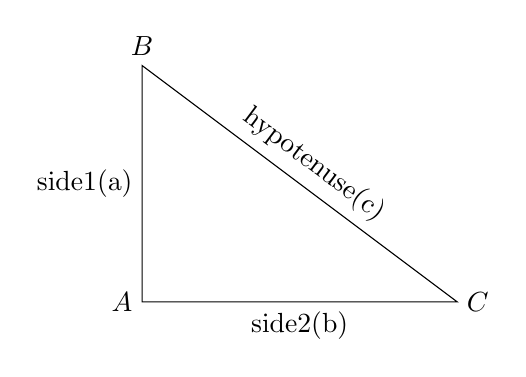
\begin{tikzpicture}[scale=1]
    \coordinate [label=left:$A$] (A) at (0, 0);
    \coordinate [label=above:$B$] (B) at (0, 3);
    \coordinate [label=right:$C$] (C) at (4, 0);
    \draw (A) -- node[left] {side1(a)}
          (B) -- node[sloped,above] {hypotenuse(c)}
          (C) -- node[below] {side2(b)} cycle;
  \end{tikzpicture}
  \begin{align*}
    c^2 = a^2 + b^2 \\
    or \\
    c = \sqrt{a^2 + b^2}
  \end{align*}
  \caption{Pythagorean Theorem}
  \label{fig:pythagorean-theorem}
\end{figure}

% Sample method for calculating the hypotenuse in the pythagorean theorem
\begin{lstlisting}[language=Java, caption={Sample Method for Calculating the Hypotenuse}, label={lst:sample-method}]
  // Hypotenuse.java
  public class Hypotenuse {
    public static void main(String[] args) {
      double side1 = 3.0;
      double side2 = 4.0;

      double hypotenuse = calculateHypotenuse(side1, side2);
      System.out.println("The hypotenuse is: " + hypotenuse);
    }

    public static double calculateHypotenuse(double side1, double side2) {
      double hypotenuse = Math.sqrt(side1 * side1 + side2 * side2);
      return hypotenuse;
    }
  }

  // Output:
  // The hypotenuse is: 5.0
\end{lstlisting}

Code \ref{lst:sample-method} shows a sample method for calculating the hypotenuse
of a right-angled triangle using the Pythagorean theorem as shown in Figure
\ref{fig:pythagorean-theorem}. The method ``calculateHypotenuse'' accepts two
parameters ``side1'' and ``side2'' which represent the two sides of the triangle.
The method calculates the hypotenuse using the formula $c = \sqrt{a^2 + b^2}$ and
returns the result. As per the example, the arguments 3.0 and 4.0 are passed to
the method to calculate the hypotenuse of the triangle.

\section{Types of Methods}

There are two types of methods in Java: predefined methods and user-defined
methods.

\subsection{Predefined Methods}

Predefined methods are built-in methods that are provided by Java. They are
available in the Java API and can be used directly in your programs. Predefined
methods are used to perform common tasks such as input/output operations,
mathematical calculations, string manipulation, and more.

% Some examples of predefined methods
\begin{lstlisting}[language=Java, caption={Examples of Predefined Methods}, label={lst:predefined-methods}]
  // Math class methods
  double squareRoot = Math.sqrt(16);
  double power = Math.pow(2, 3);
  double absoluteValue = Math.abs(-5);

  // String class methods
  String str = "Hello, World!";
  int length = str.length();
  String upperCase = str.toUpperCase();
  String lowerCase = str.toLowerCase();
\end{lstlisting}

Code \ref{lst:predefined-methods} shows examples of predefined methods in Java.
The ``Math'' class provides methods for mathematical calculations such as
calculating the square root, power, and absolute value of a number. The ``String''
class provides methods for string manipulation such as getting the length of a
string, converting a string to uppercase, and converting a string to lowercase.

\subsection{User-Defined Methods}

User-defined methods are methods that are created by the programmer to perform
specific tasks. They are defined within a class and can be called from other
parts of the program. User-defined methods are used to organize code, make it
reusable, and reduce redundancy.

% Sample user-defined methods
\begin{lstlisting}[language=Java, caption={Sample User-Defined Methods}, label={lst:user-defined-methods}]
  // UserDefinedMethods.java
  public class UserDefinedMethods {
    public static void main(String[] args) {
      float  areaEllipse = calculateAreaEllipse(3, 4);
      System.out.println("Area of Ellipse: " + areaEllipse);

      String reversedString = reverseString("Hello, World!");
      System.out.println("Reversed String: " + reversedString);
    }

    public static float calculateAreaEllipse(float a, float b) {
      return (float) (Math.PI * a * b);
    }

    public static String reverseString(String str) {
      String reversed = "";
      for (int i = str.length() - 1; i >= 0; i--) {
        reversed += str.charAt(i);
      }
      return reversed;
    }
  }

  // Output:
  // Area of Ellipse: 37.699112
  // Reversed String: !dlroW ,olleH
\end{lstlisting}

Code \ref{lst:user-defined-methods} shows examples of user-defined methods in Java.
The ``calculateFactorial'' method calculates the factorial of a number using a
``for'' loop. The ``reverseString'' method reverses a string by iterating over
the characters of the string in reverse order.

\section{Static Methods}

A static method is a method that belongs to the class rather than an instance
of the class. It can be called directly using the class name without creating
an object of the class. Static methods are used for utility functions that do
not require access to instance variables.

% Sample static method
\begin{lstlisting}[language=Java, caption={Sample Static Method}, label={lst:static-method}]
  // StaticMethod.java
  public class StaticMethod {
    public static void main(String[] args) {
      Person person1 = new Person("Alice", 25);
      Person person2 = new Person("Bob", 30);

      int countPersons = Person.getCountPersons();
      System.out.println("Number of Persons: " + countPersons);
    }
  }

  // Person.java
  public class Person {
    private String name;
    private int age;
    private static int count = 0;

    public Person(String name, int age) {
      this.name = name;
      this.age = age;
      count++;
    }

    public String getName() {
      return name;
    }

    public int getAge() {
      return age;
    }

    public static int getCountPersons() {
      return count;
    }
  }
  
  // Output:
  // Number of Persons: 2
\end{lstlisting}
  
Code \ref{lst:static-method} shows an example of a static method in Java. The
``Person'' class has a static method ``getCountPersons'' that returns the number
of instances of the ``Person'' class. The static method can be called using the
class name ``Person'' without creating an object of the class.

\section{Method Overloading}

Method overloading is a feature that allows a class to have multiple methods
with the same name but different parameters. It is used to provide different
implementations of a method based on the number or type of parameters.

% Sample method overloading
\begin{lstlisting}[language=Java, caption={Sample Method Overloading}, label={lst:method-overloading}]
  // MethodOverloading.java
  public class MethodOverloading {
    public static void main(String[] args) {
      int sum1 = add(1, 2);
      int sum2 = add(1, 2, 3);
      double sum3 = add(1.5, 2.5);

      System.out.println("Sum of 1 and 2: " + sum1);
      System.out.println("Sum of 1, 2, and 3: " + sum2);
      System.out.println("Sum of 1.5 and 2.5: " + sum3);
    }

    public static int add(int a, int b) {
      return a + b;
    }

    public static int add(int a, int b, int c) {
      return a + b + c;
    }

    public static double add(double a, double b) {
      return a + b;
    }
  }

  // Output:
  // Sum of 1 and 2: 3
  // Sum of 1, 2, and 3: 6
  // Sum of 1.5 and 2.5: 4.0
\end{lstlisting}

Code \ref{lst:method-overloading} shows an example of method overloading in Java.
The ``add'' method is overloaded to accept different numbers of parameters and
different types of parameters. The method can be called with two integers, three
integers, or two doubles.

\section{Recursion}

Recursion is a programming technique in which a method calls itself to solve
a problem. It is used to break down a complex problem into smaller subproblems
that are easier to solve. Recursion consists of two parts: the base case and
the recursive case. The base case is the condition that stops the recursion,
while the recursive case is the condition that calls the method recursively.

% Sample recursive method
\begin{lstlisting}[language=Java, caption={Sample Recursive Method}, label={lst:recursive-method}]
  // RecursiveMethod.java
  public class RecursiveMethod {
    public static void main(String[] args) {
      int factorial = calculateFactorial(5);
      System.out.println("Factorial of 5: " + factorial);
    }

    public static int calculateFactorial(int n) {
      if (n == 0) {
        return 1;
      } else {
        return n * calculateFactorial(n - 1);
      }
    }
  }

  // Output:
  // Factorial of 5: 120
\end{lstlisting}

Code \ref{lst:recursive-method} shows an example of a recursive method in Java.
The ``calculateFactorial'' method calculates the factorial of a number using
recursion. The base case is when the number is 0, in which case the method
returns 1. The recursive case is when the number is greater than 0, in which
case the method calls itself with the number decremented by 1.

% Draw a diagram showing the recursive calls for calculating the factorial of 5
\begin{figure}[h]
  \centering
  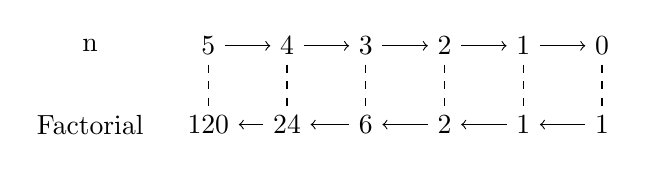
\begin{tikzpicture}[scale=1]
    \node (nbegin) at (-1.5, 0) {n};
    \node (n5) at (0, 0) {5};
    \node (n4) at (1, 0) {4};
    \node (n3) at (2, 0) {3};
    \node (n2) at (3, 0) {2};
    \node (n1) at (4, 0) {1};
    \node (n0) at (5, 0) {0};
    
    \node (r0) at (5, -1) {1};
    \node (r1) at (4, -1) {1};
    \node (r2) at (3, -1) {2};
    \node (r3) at (2, -1) {6};
    \node (r4) at (1, -1) {24};
    \node (r5) at (0, -1) {120};
    \node (rend) at (-1.5, -1) {Factorial};

    \draw[->] (n5) -- (n4);
    \draw[->] (n4) -- (n3);
    \draw[->] (n3) -- (n2);
    \draw[->] (n2) -- (n1);
    \draw[->] (n1) -- (n0);

    \draw[dashed] (n0) -- (r0);
    \draw[dashed] (n1) -- (r1);
    \draw[dashed] (n2) -- (r2);
    \draw[dashed] (n3) -- (r3);
    \draw[dashed] (n4) -- (r4);
    \draw[dashed] (n5) -- (r5);

    \draw[->] (r0) -- (r1);
    \draw[->] (r1) -- (r2);
    \draw[->] (r2) -- (r3);
    \draw[->] (r3) -- (r4);
    \draw[->] (r4) -- (r5);
  \end{tikzpicture}
  \caption{Recursive Calls for Calculating the Factorial of 5}
  \label{fig:recursive-calls}
\end{figure}

Figure \ref{fig:recursive-calls} shows the recursive calls for calculating the
factorial of 5 using the ``calculateFactorial'' method. The method is called
repeatedly with decreasing values of ``n'' until the base case is reached.

\section{Summary}

A \textbf{Method} is a block of code that performs a specific task. It is used
to organize code, make it reusable, and reduce redundancy. Methods are declared
using an access modifier, return type, method name, parameter list, and method
body. Methods can be called using the method name followed by parentheses.

\textbf{Parameters} are variables that are used to pass values to a method.
They are specified in the method declaration and act as placeholders for the
values that are passed to the method. \textbf{Arguments} are the actual values
that are passed to the method when it is called.

There are two types of methods in Java: predefined methods and user-defined
methods. \textbf{Predefined methods} are built-in methods provided by Java
for common tasks such as input/output operations, mathematical calculations,
and string manipulation. \textbf{User-defined methods} are methods created by
the programmer to perform specific tasks.

A \textbf{static method} is a method that belongs to the class rather than an
instance of the class. It can be called directly using the class name without
creating an object of the class. Static methods are used for utility functions
that do not require access to instance variables.

\textbf{Method overloading} is a feature that allows a class to have multiple
methods with the same name but different parameters. It is used to provide
different implementations of a method based on the number or type of parameters.

\textbf{Recursion} is a programming technique in which a method calls itself
to solve a problem. It is used to break down a complex problem into smaller
subproblems that are easier to solve. Recursion consists of two parts: the
base case and the recursive case.

%%%%%%%%%%%%%%%%%%%%%%%
%%%     Chapter     %%%
%%%%%%%%%%%%%%%%%%%%%%%
\chapter{Classes and Objects}

\section{Introduction to Classes and Objects}

\section{Declaration, Initialization, and Instantiation}

\section{Constructors}

\subsection{Default Constructor}

\subsection{Parameterized Constructor}

\subsection{Constructor Overloading}

\section{Summary}

%%%%%%%%%%%%%%%%%%%%%%%
%%%     Chapter     %%%
%%%%%%%%%%%%%%%%%%%%%%%
\chapter{Four Pillars of Object-Oriented Programming}

\section{Inheritance}

\section{Polymorphism}

\section{Encapsulation}

\section{Abstraction}

\section{Typecasting}

\subsection{Downcasting}

\subsection{Upcasting}

\section{Summary}

%%%%%%%%%%%%%%%%%%%%%%%
%%%     Chapter     %%%
%%%%%%%%%%%%%%%%%%%%%%%
\chapter{Composition and Enumeration}

\section{Relationships Between Classes}

\section{Composition}

\section{Enumeration}

\section{Summary}

%%%%%%%%%%%%%%%%%%%%%%%
%%%     Chapter     %%%
%%%%%%%%%%%%%%%%%%%%%%%
% \chapter{Exception Handling and Unit Testing}

% \section{Types of Exceptions}

% \section{Try-Catch Block}

% \section{Exception Throwing and Propagation}

% \section{Unit Testing}

% \section{Summary}

%%%%%%%%%%%%%%%%%%%%%%%
%%%     Chapter     %%%
%%%%%%%%%%%%%%%%%%%%%%%
\chapter{Coding Guidelines and Best Practices}

\section{Naming Conventions}

\section{Code Formatting}

\section{Documentation}

\section{Code Maintainability}

\section{Summary}

\chapter{References}

\begin{enumerate}[label={\Alph*.}]
  \item \textbf{Books}
    \begin{itemize}
      \item Loy, M., Niemeyer, P., \& Leuck, D. (2023). \textit{Learning Java: An Introduction to Real-World Programming with Java}. O’Reilly Media. ISBN: 9781098145538
      \item Horstmann, C. S. (2022). \textit{Core Java, Volume I: Fundamentals}. Pearson Education. ISBN: 978-0137673629
      \item Schildt, H. (2022). \textit{Java: The Complete Reference, Twelfth Edition}. McGraw Hill Professional. ISBN: 978-1-260-46341-5
      \item Schildt, H. (2022). \textit{Java: A Beginner’s Guide, Ninth Edition}. McGraw Hill Professional. ISBN: 978-1-260-46355-2
      \item Paul Deitel \& Harvey Deitel (July 14th 2021). \textit{Java: How To Program, Early Objects, 11th edition}. Deitel \& Associates, Inc. ISBN: 13:9780137505166
      \item Cay S. Horstmann (2019). \textit{Brief Java: early objects 9th edition}. Wiley. ISBN: 978-1-119-49913-8
      \item Chemuturi, M. (2019). \textit{Computer Programming for Beginners: A Step-By-Step Guide}. Chapman and Hall/CRC. ISBN: 978-1138320482
      \item Chua (2019). \textit{Intermediate Programming Using C}. ISBN: 13 987-1498711630
    \end{itemize}
  \item \textbf{Other Sources}
    \begin{itemize}
      \item \textnormal{GeeksforGeeks (2022). \textit{Object Oriented Programming (OOPs) Concept in Java}. GeeksforGeeks. https://www.geeksforgeeks.org/object-oriented-programming-oops-concept-in-java/}
      \item \textnormal{JavaTpoint (2022). \textit{Java OOPs Concepts}. JavaTpoint. https://www.javatpoint.com/java-oops-concepts}
      \item \textnormal{Tutorialspoint (2019). \textit{Java Tutorial}. Tutorialspoint. https://www.tutorialspoint.com/java/index.htm}
      \item \textnormal{W3Schools (2019). \textit{Java Tutorial}. W3Schools. https://www.w3schools.com/java/}
    \end{itemize}
\end{enumerate}

\end{document}
